% Лабораторная работа по АСиСу № 8
% Михедов Константин Константинович

% Тип документа: статья, на бумаге А4
\documentclass[a4paper]{article}

% Подключение сторонних tex файлов 
\usepackage{import}


% Основные данные - ВУЗ, факультет, город...
\import{./../../stuff/tex}{config.tex}

% Подключение необходимых зависимостей
\import{./../../stuff/tex/settings}{packages.tex}
% Настройка подключенных пакетов
\import{./../../stuff/tex/settings}{preferences.tex}


% Шаблон титульной страницы 
\import{./../../stuff/tex/templates}{title.tex}
% Упрощенный блок "выполнил"
\import{./../../stuff/tex/templates}{sign1.tex}
% Макрос для содержания
\import{./../../stuff/tex/templates}{toc.tex}

% Определяем название документа
\title{
  Лабораторная работа №8 по курсу \\
  <<Компьютерный практикум <<Администрирование систем и сетей>>  
}
% Отключаем отображение правительства
\renewcommand{\government}{}
% Отключаем сокращенное нзавание университета
\renewcommand{\subuniversity}{}
% Указываем преподавателя
\renewcommand{\shortteachername}{Зудин Д.Е.}


% Путь до внешних изображений
\graphicspath{ {./figures/}}


% Основной текст работы
\begin{document}
  \templatedtitlepage
  
  \toc
  \section{Ход работы}

  Все имена выбраны в соответсвии с 9 вариантом.

  \subsection{Настройка сети}

  Для выполнения данной работы потребуются две виртуальные машины,
  объединенные в одну \textit{NAT} сеть (имеется доступ в Интернет).
  Создадим такую сеть:

  \begin{figure}[H]
    \centering
    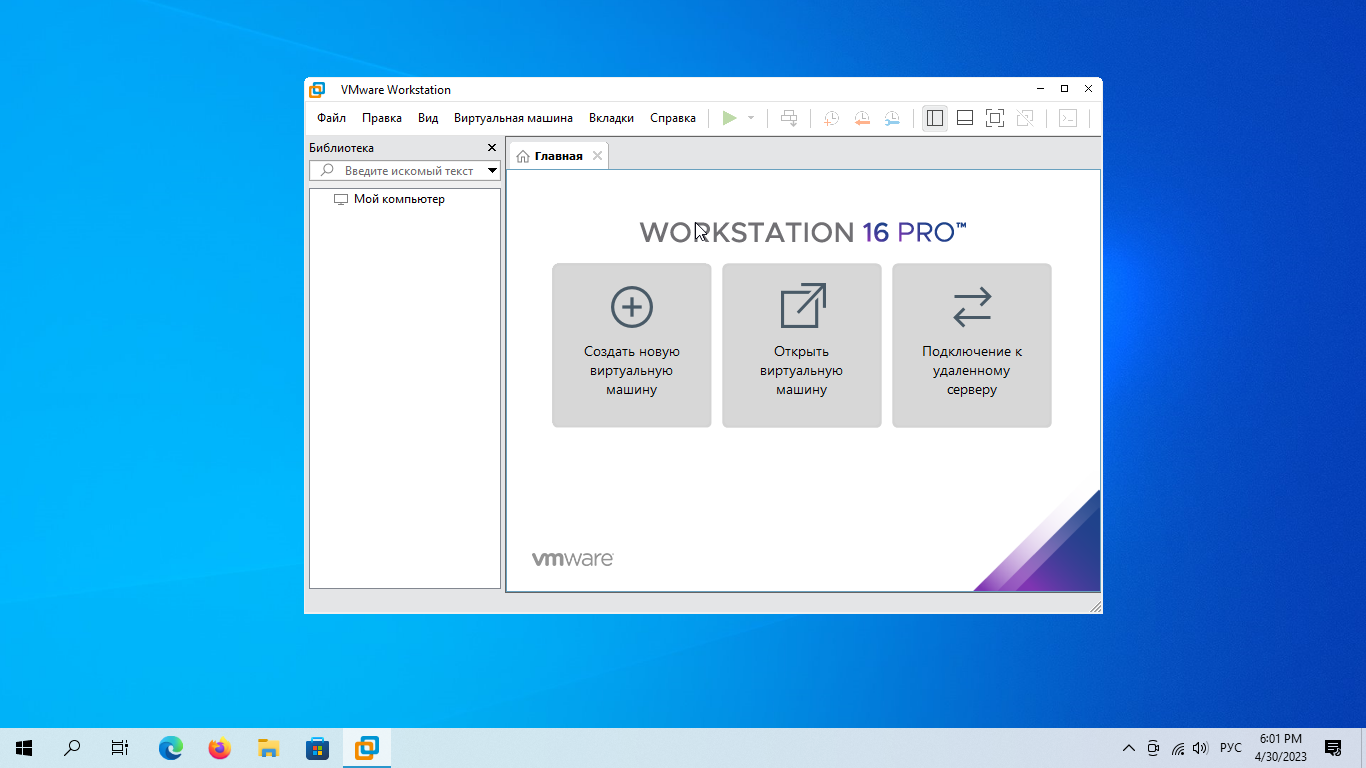
\includegraphics[width=0.85\textwidth]{Screenshot_1}
    \caption{Запускаем VMware}
    \label{img:1}
  \end{figure}

  \begin{figure}[H]
    \centering
    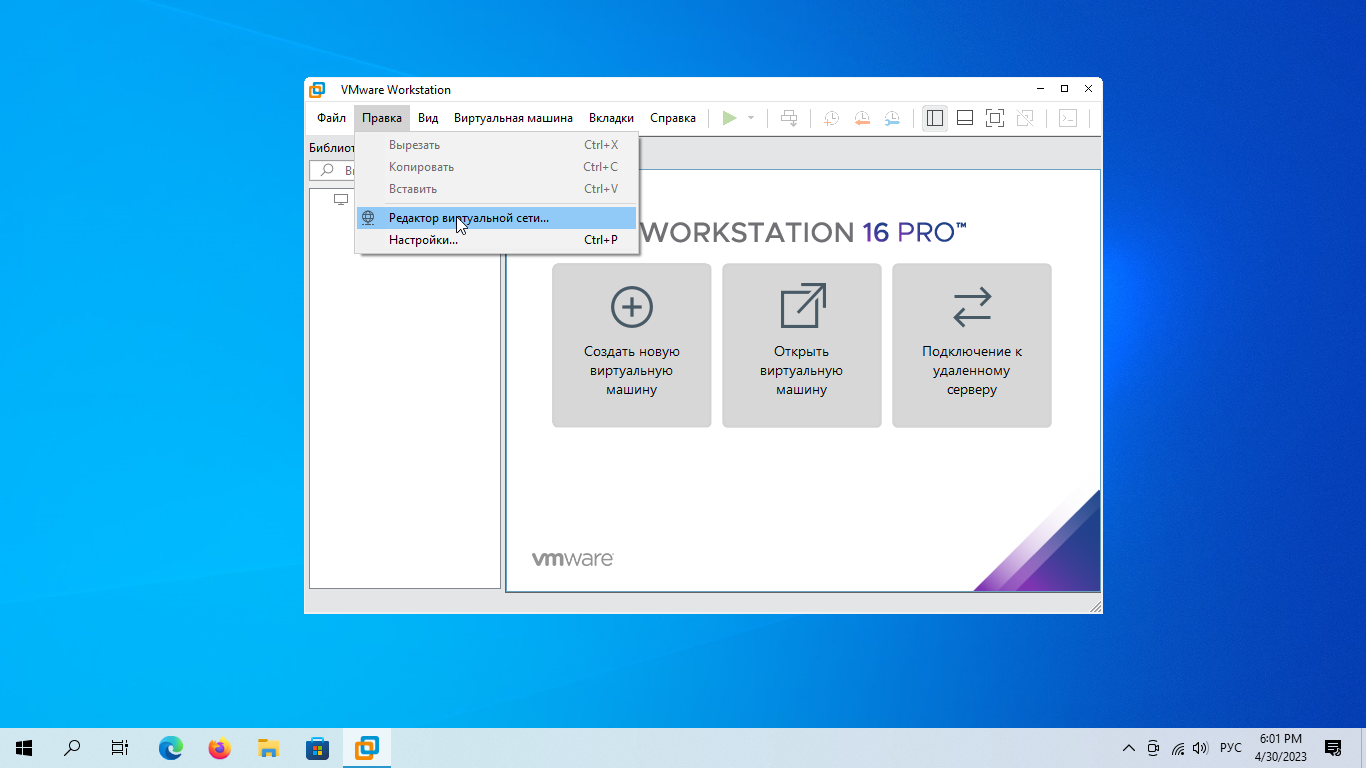
\includegraphics[width=0.85\textwidth]{Screenshot_2}
    \caption{Открываем редактор виртуальной сети}
    \label{img:2}
  \end{figure}

  \begin{figure}[H]
    \centering
    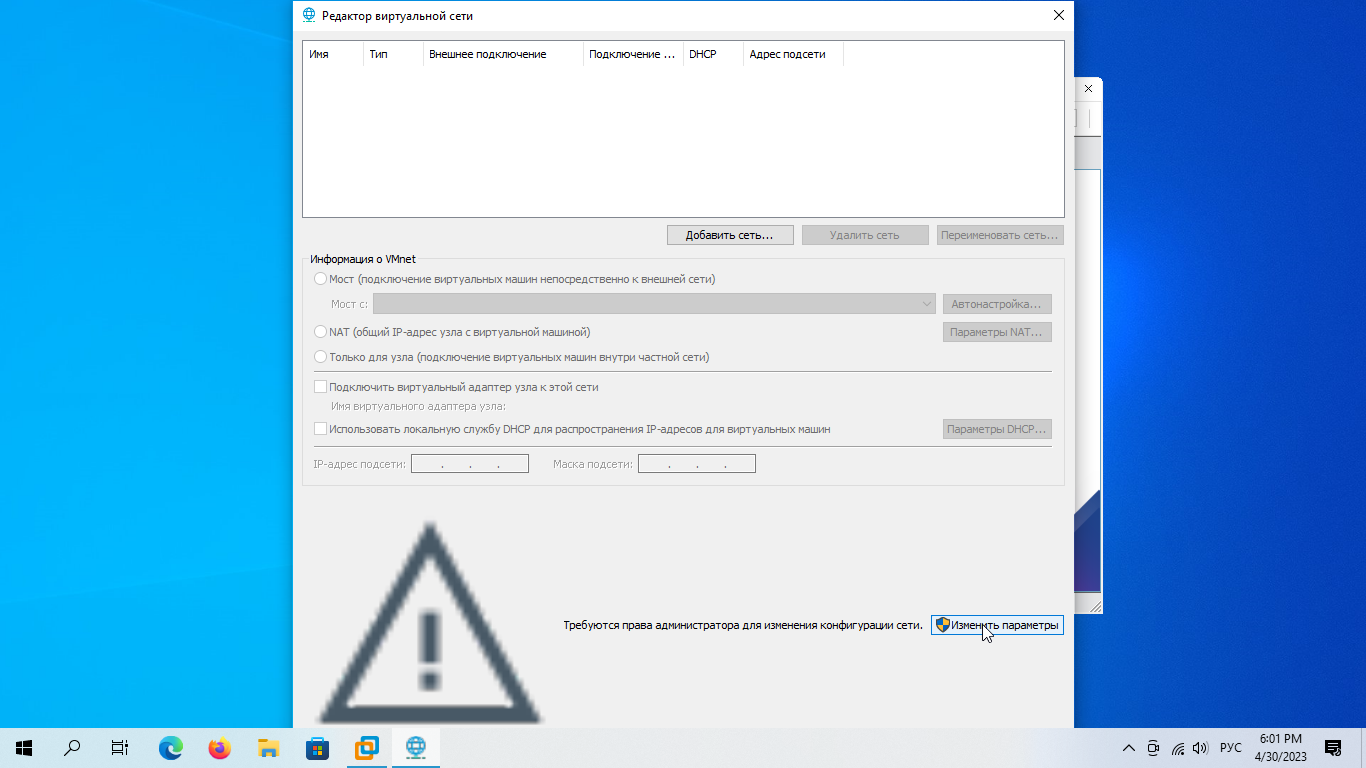
\includegraphics[width=0.85\textwidth]{Screenshot_3}
    \caption{Выдаем программе права администратора, чтобы было стало возможным менять системные параметры}
    \label{img:3}
  \end{figure}

  Предыдущий шаг необходим, так как \textit{VMware} создает виртуальные адаптеры,
  к которым подключает хостовую машину. Это требует изменений системной конфигурации,
  для которых как раз и необходимы права администратора.

  \begin{figure}[H]
    \centering
    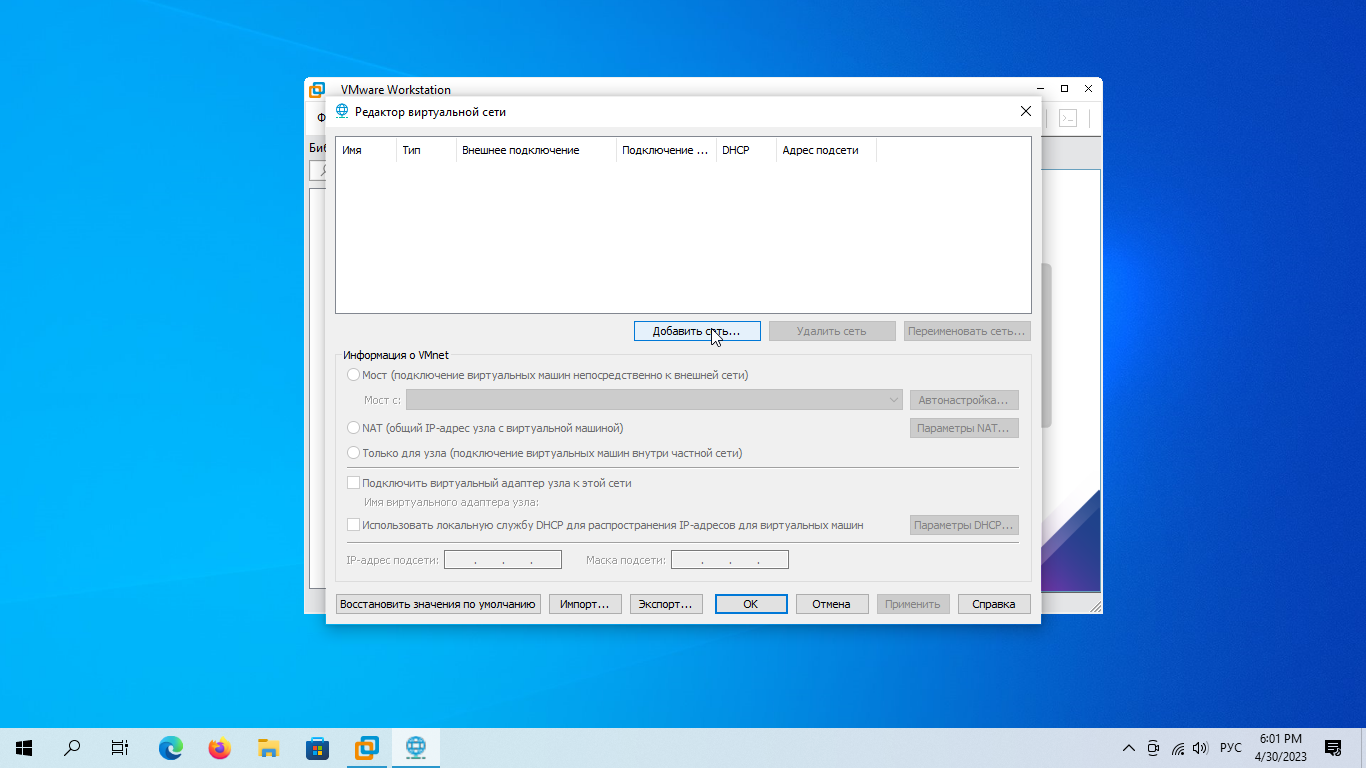
\includegraphics[width=0.85\textwidth]{Screenshot_4}
    \caption{Начинаем добавление новой сети}
    \label{img:4}
  \end{figure}

  \begin{figure}[H]
    \centering
    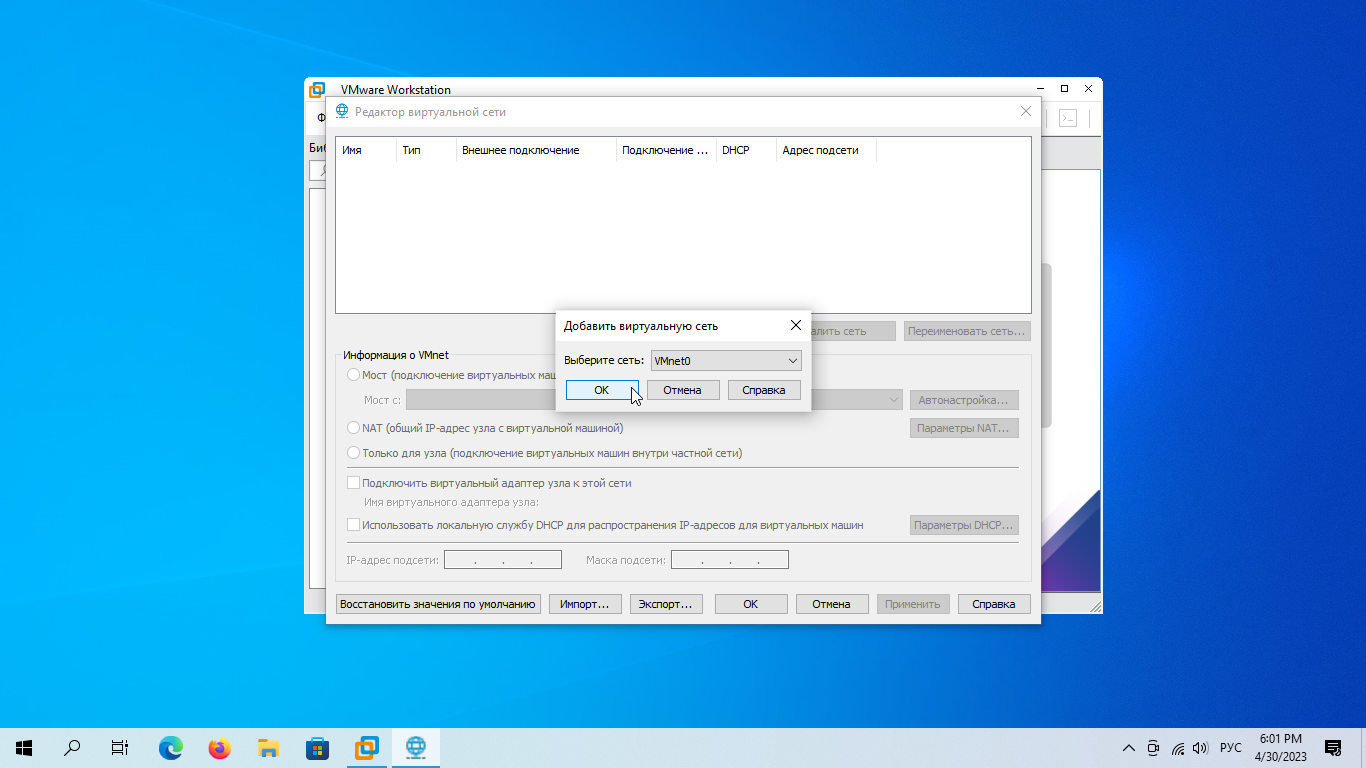
\includegraphics[width=0.85\textwidth]{Screenshot_5}
    \caption{Выбираем имя новой сети - \textit{VMnet0}}
    \label{img:5}
  \end{figure}

  \begin{figure}[H]
    \centering
    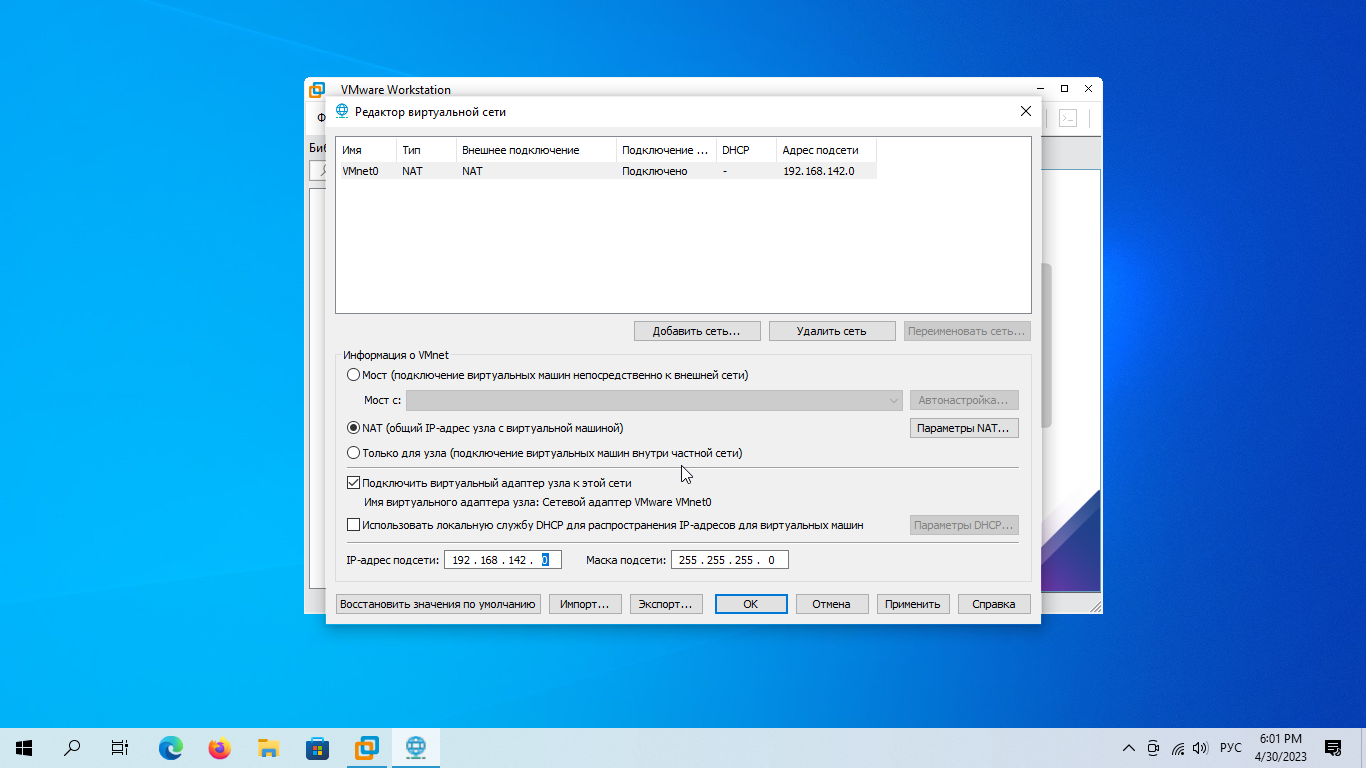
\includegraphics[width=0.85\textwidth]{Screenshot_6}
    \caption{Указываем тип и параметры сети}
    \label{img:6}
  \end{figure}

  Наиболее важным является тип сети - \textit{NAT}. Такая сеть позволит виртуальным машинам
  осуществлять доступ в Интернет. Также необходимо отключить встроенный \textit{DHCP}-сервер,
  так как назначение \textit{IP} адресов будет происходить вручную (статическая адресация).

  В качестве адреса сети был выбран 192.168.142.0/24.

  \begin{figure}[H]
    \centering
    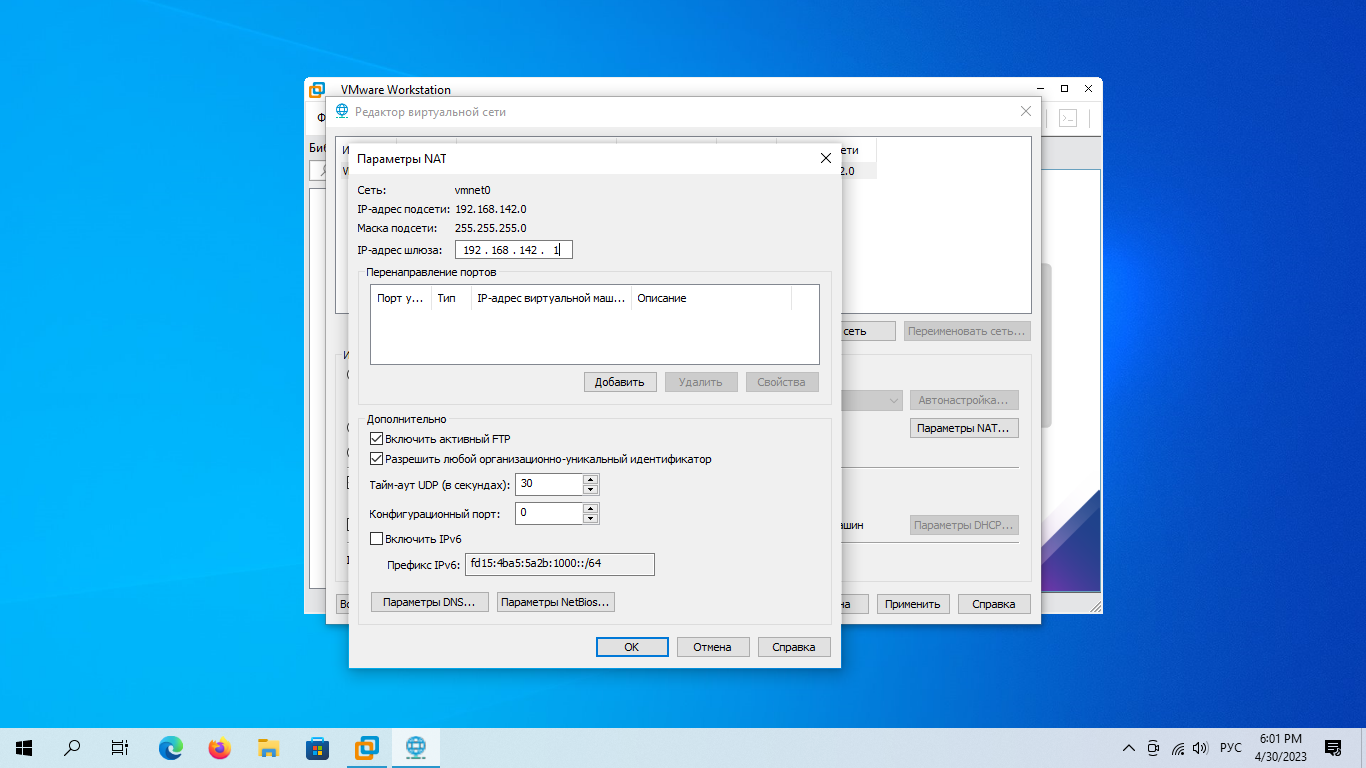
\includegraphics[width=0.85\textwidth]{Screenshot_7}
    \caption{Открываем параметры \textit{NAT}}
    \label{img:7}
  \end{figure}

  Так как адрес сети был выбран мной, а не назначен автоматически, необходимо
  также вручную указать \textit{IP} адрес шлюза по умолчанию. Возьмем первый доступный
  - 192.168.142.1. Этот же адрес можно будет использовать как первичный \textit{DNS}.

  \begin{figure}[H]
    \centering
    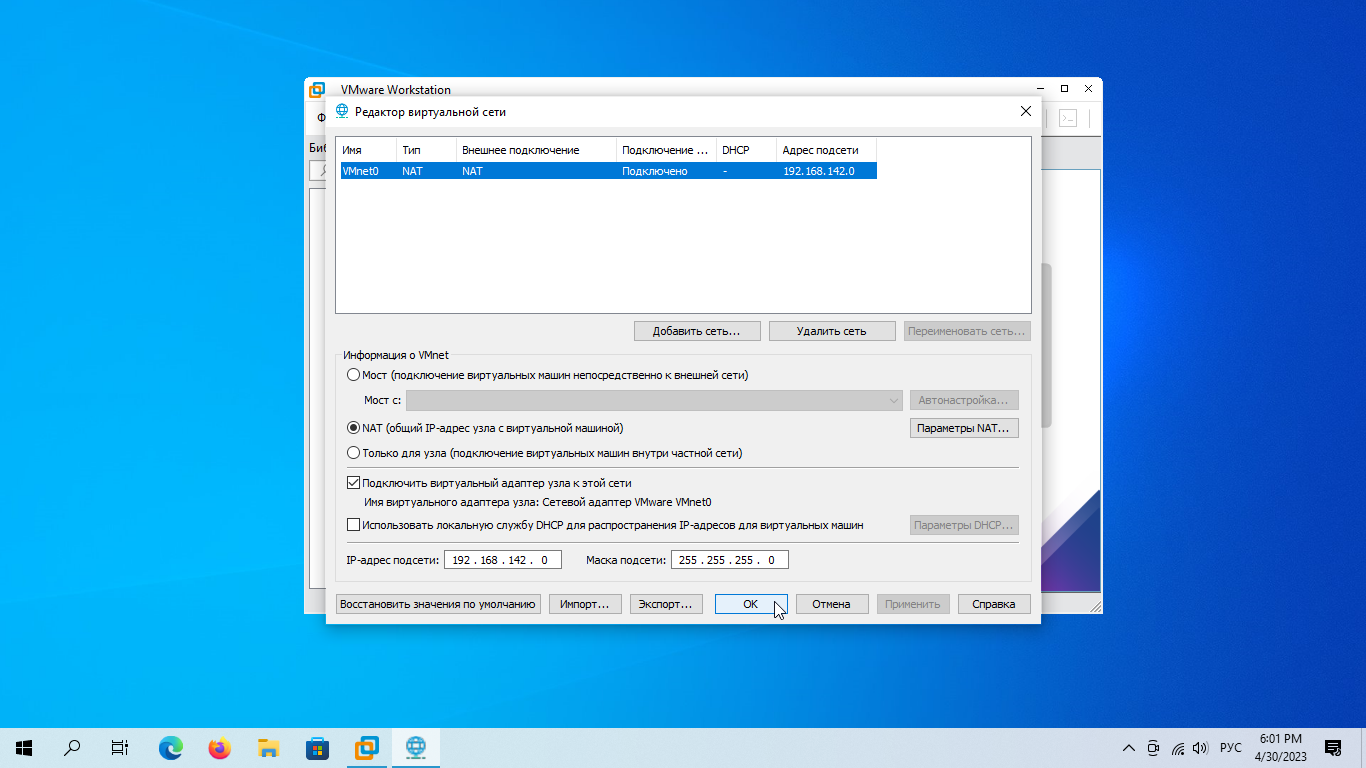
\includegraphics[width=0.85\textwidth]{Screenshot_8}
    \caption{Сеть создана и настроена - применяем новые параметры}
    \label{img:8}
  \end{figure}

  \subsection{Настройка Windows Server 2016}

  \subsubsection{Создание виртуальной машины}

  Для создания виртуальной машины с Windows Server будем использовать уже готовый образ,
  его нужно только открыть:

  \begin{figure}[H]
    \centering
    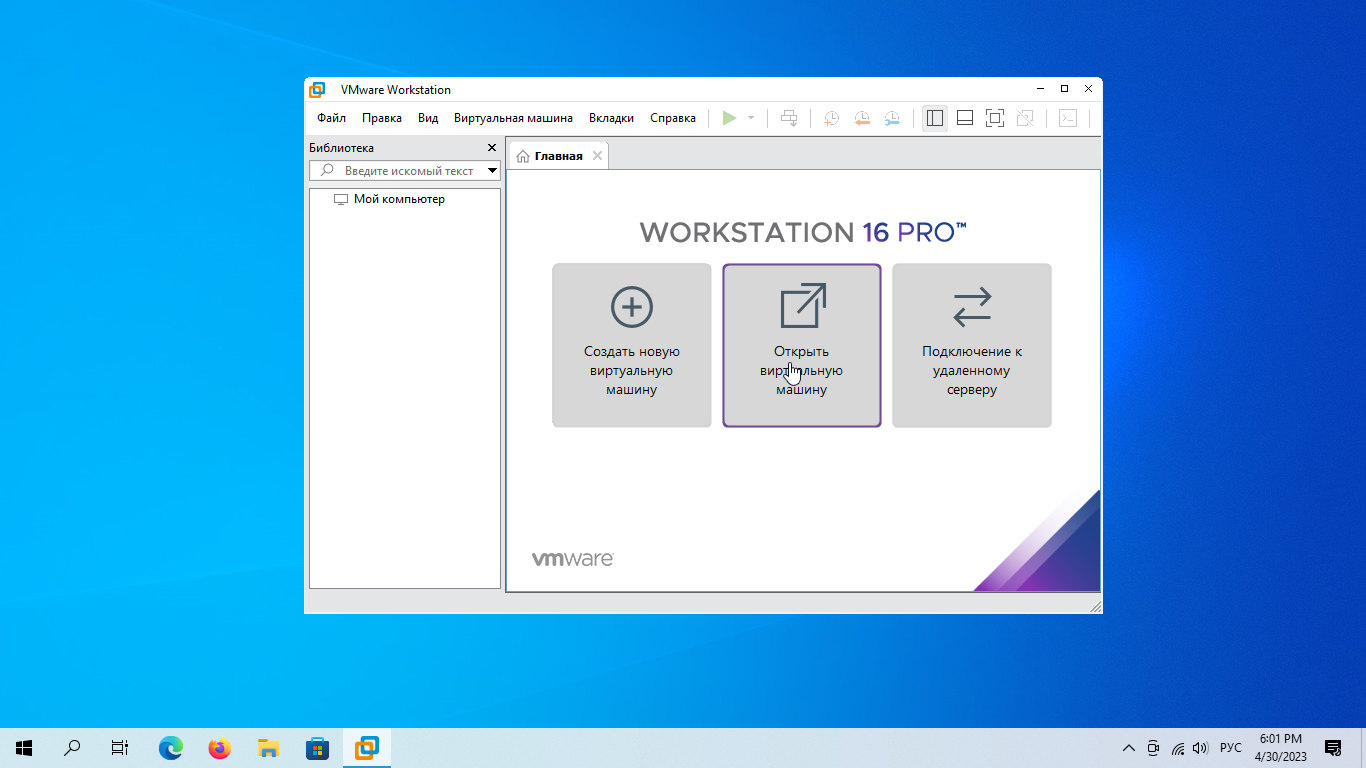
\includegraphics[width=0.85\textwidth]{Screenshot_9}
    \caption{Начинаем импорт готового образа}
    \label{img:9}
  \end{figure}

  \begin{figure}[H]
    \centering
    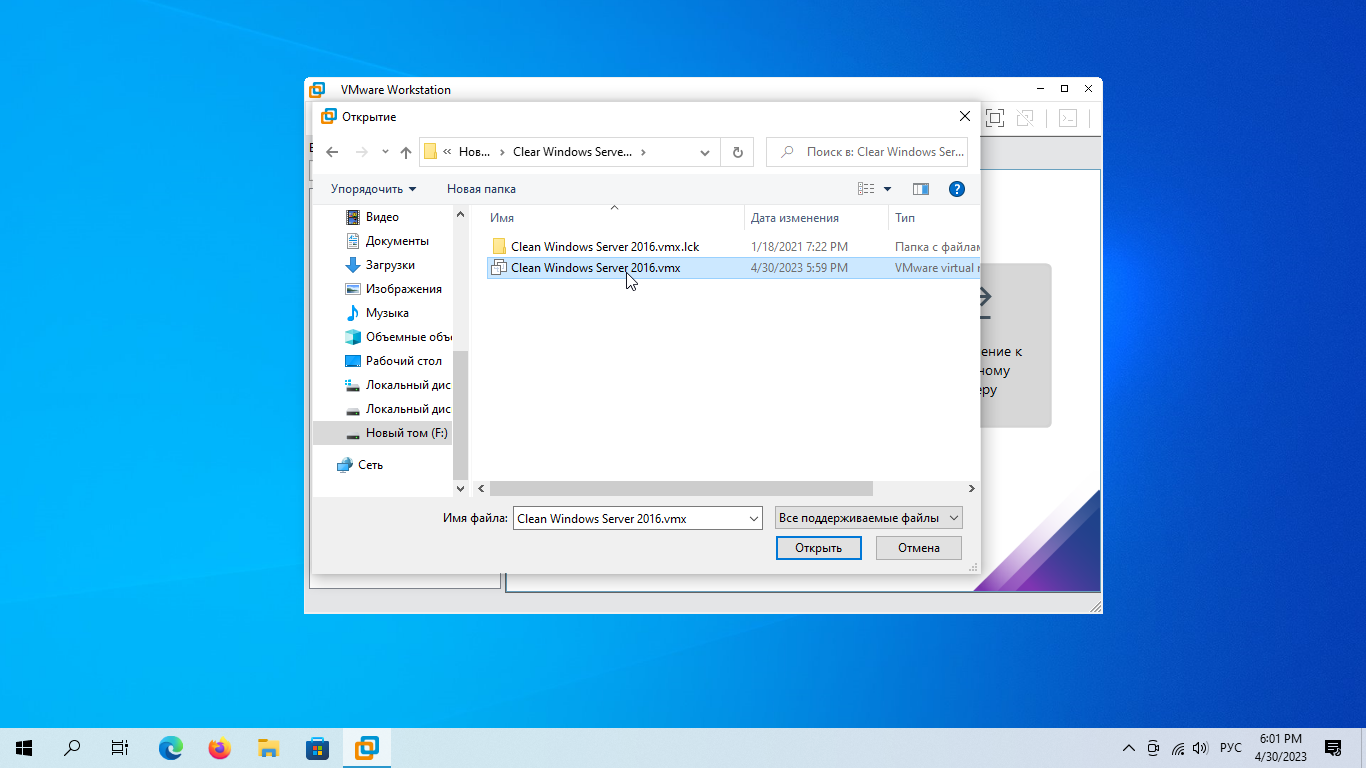
\includegraphics[width=0.85\textwidth]{Screenshot_11}
    \caption{Указываем путь до образа}
    \label{img:11}
  \end{figure}

  Теперь образ импортирован, осталось только подключить ВМ к нужной сети:

  \begin{figure}[H]
    \centering
    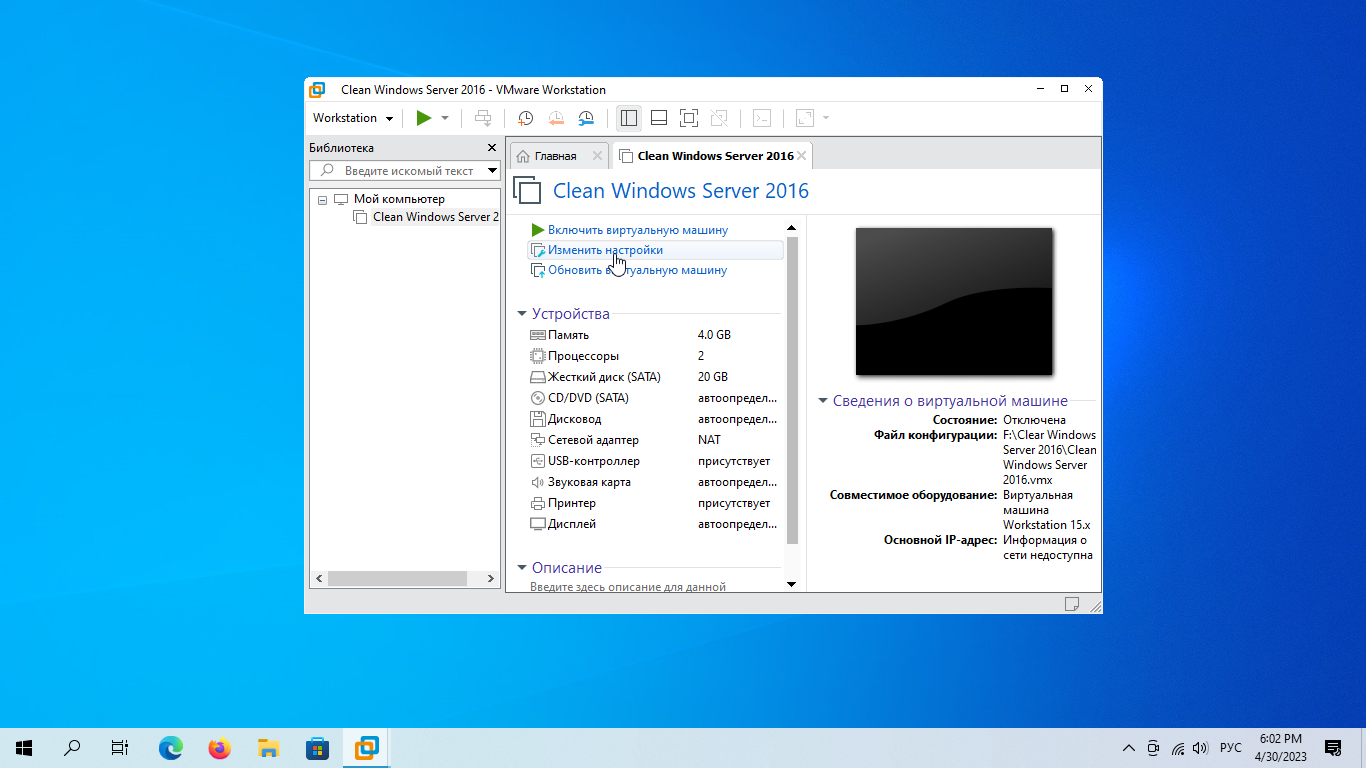
\includegraphics[width=0.85\textwidth]{Screenshot_12}
    \caption{Открываем настройки ВМ}
    \label{img:12}
  \end{figure}

  \begin{figure}[H]
    \centering
    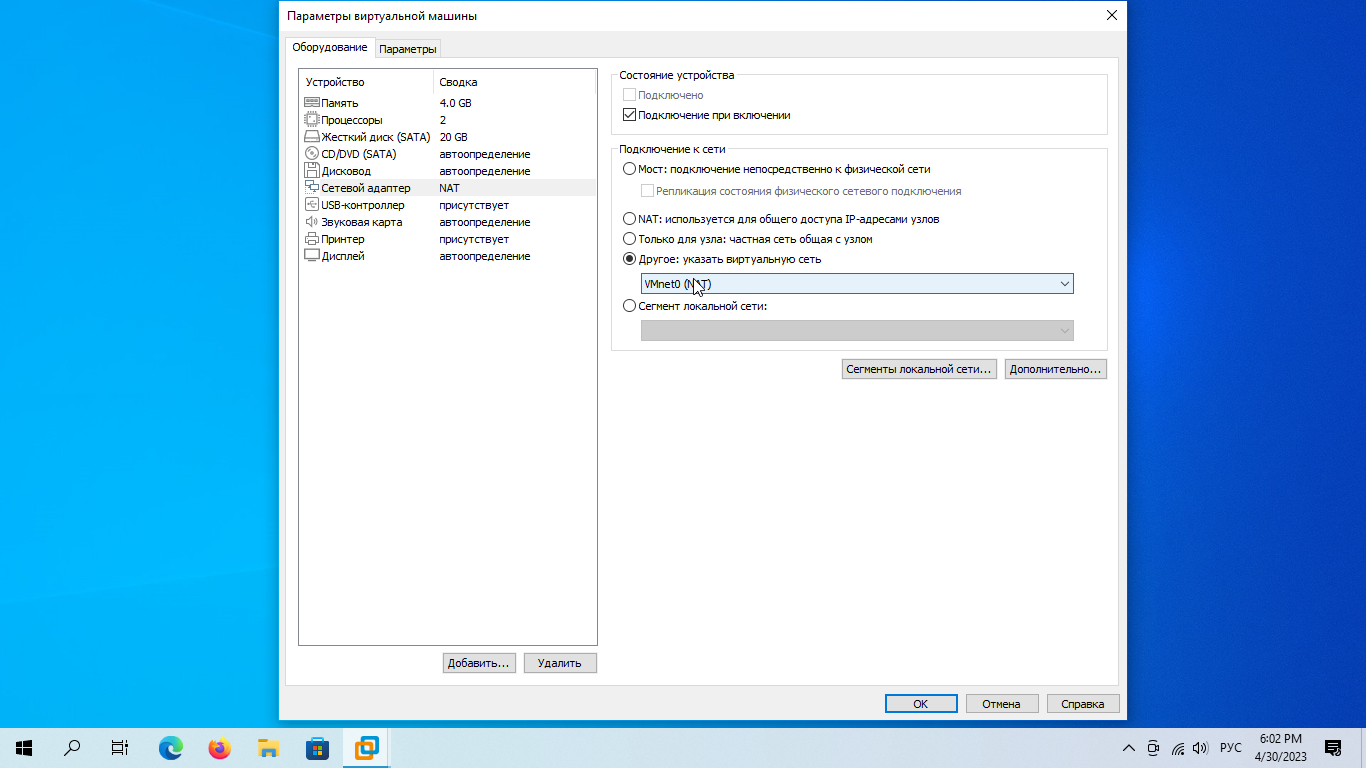
\includegraphics[width=0.85\textwidth]{Screenshot_13}
    \caption{Подключаем сетевой адаптер к созданной сети}
    \label{img:13}
  \end{figure}

  \begin{figure}[H]
    \centering
    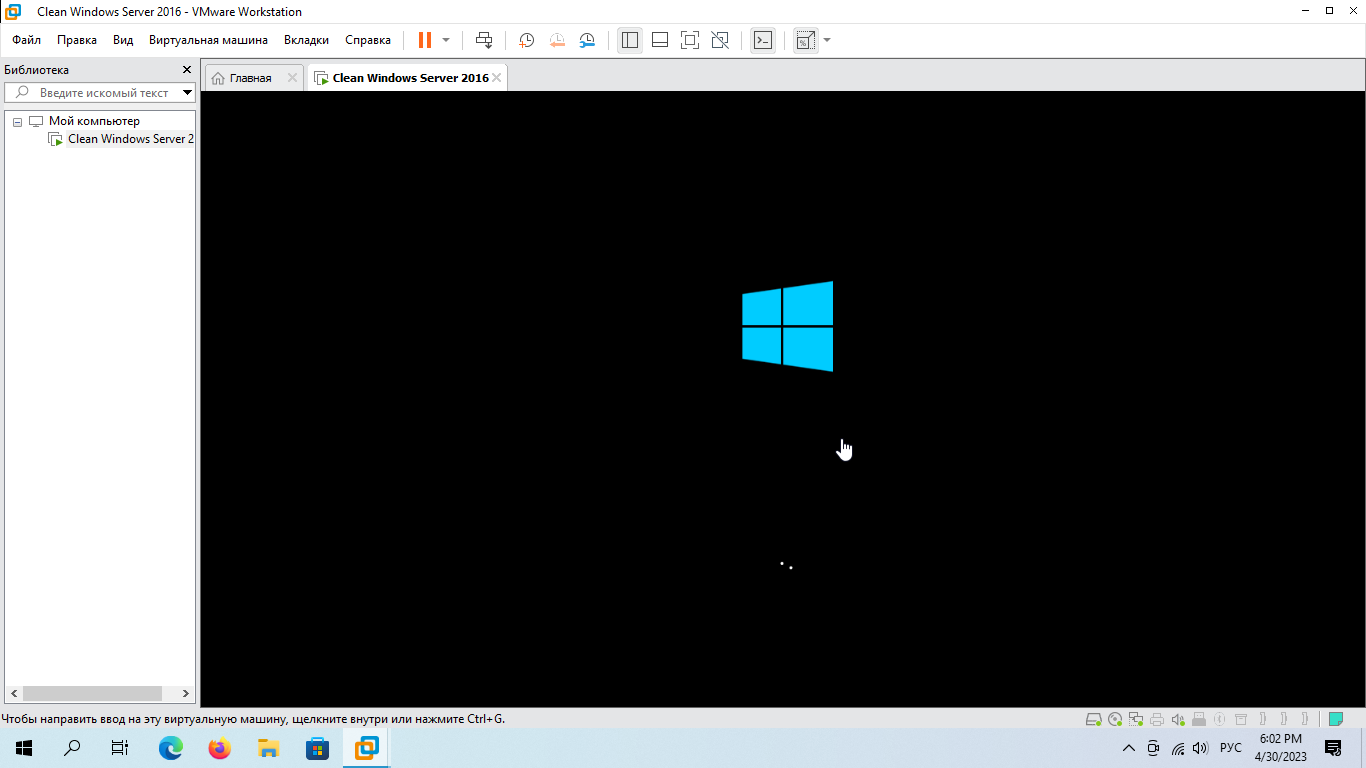
\includegraphics[width=0.85\textwidth]{Screenshot_15}
    \caption{Запускаем ВМ}
    \label{img:15}
  \end{figure}

  \subsubsection{Настройка сети}

  \begin{figure}[H]
    \centering
    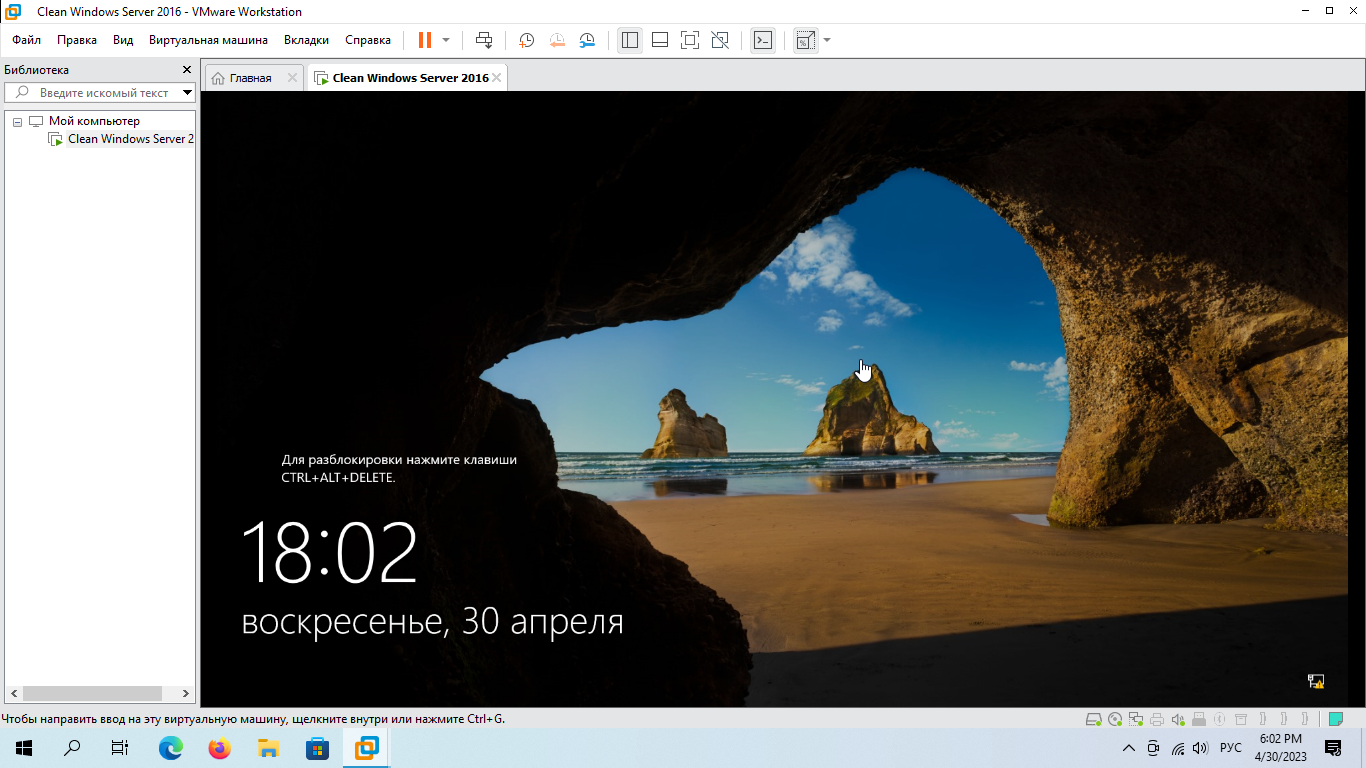
\includegraphics[width=0.85\textwidth]{Screenshot_16}
    \caption{Система загрузилась}
    \label{img:16}
  \end{figure}

  \begin{figure}[H]
    \centering
    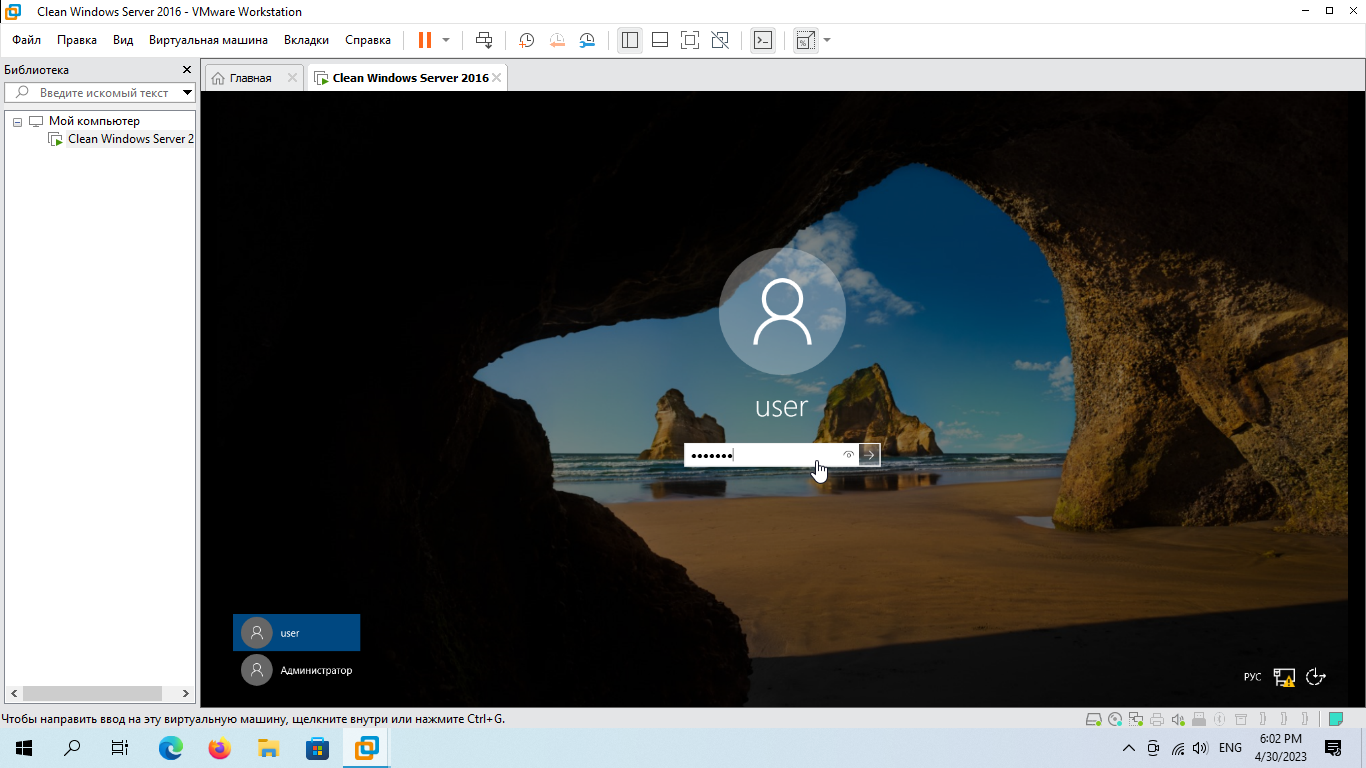
\includegraphics[width=0.85\textwidth]{Screenshot_17}
    \caption{Входим в учетную запись пользователя}
    \label{img:17}
  \end{figure}

  \begin{figure}[H]
    \centering
    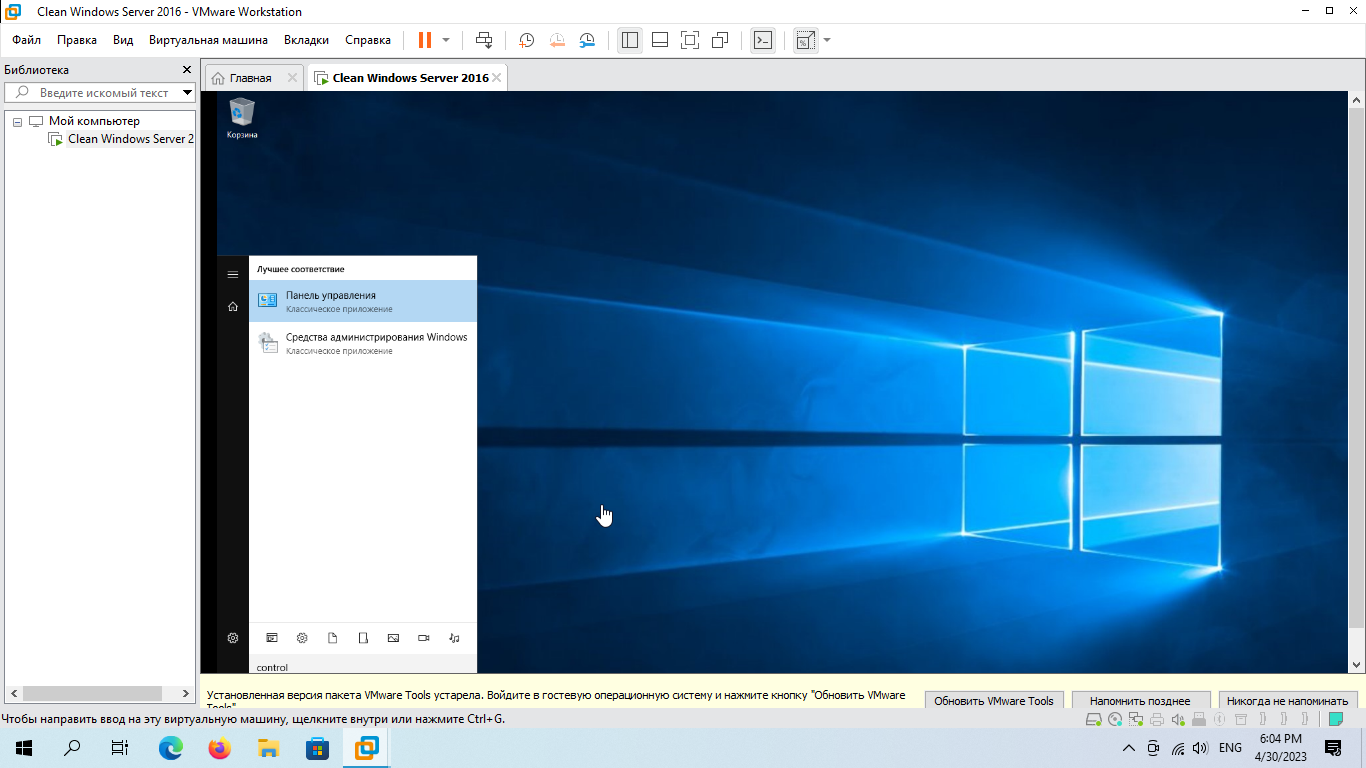
\includegraphics[width=0.85\textwidth]{Screenshot_18}
    \caption{Открываем Панель Управления}
    \label{img:18}
  \end{figure}

  \begin{figure}[H]
    \centering
    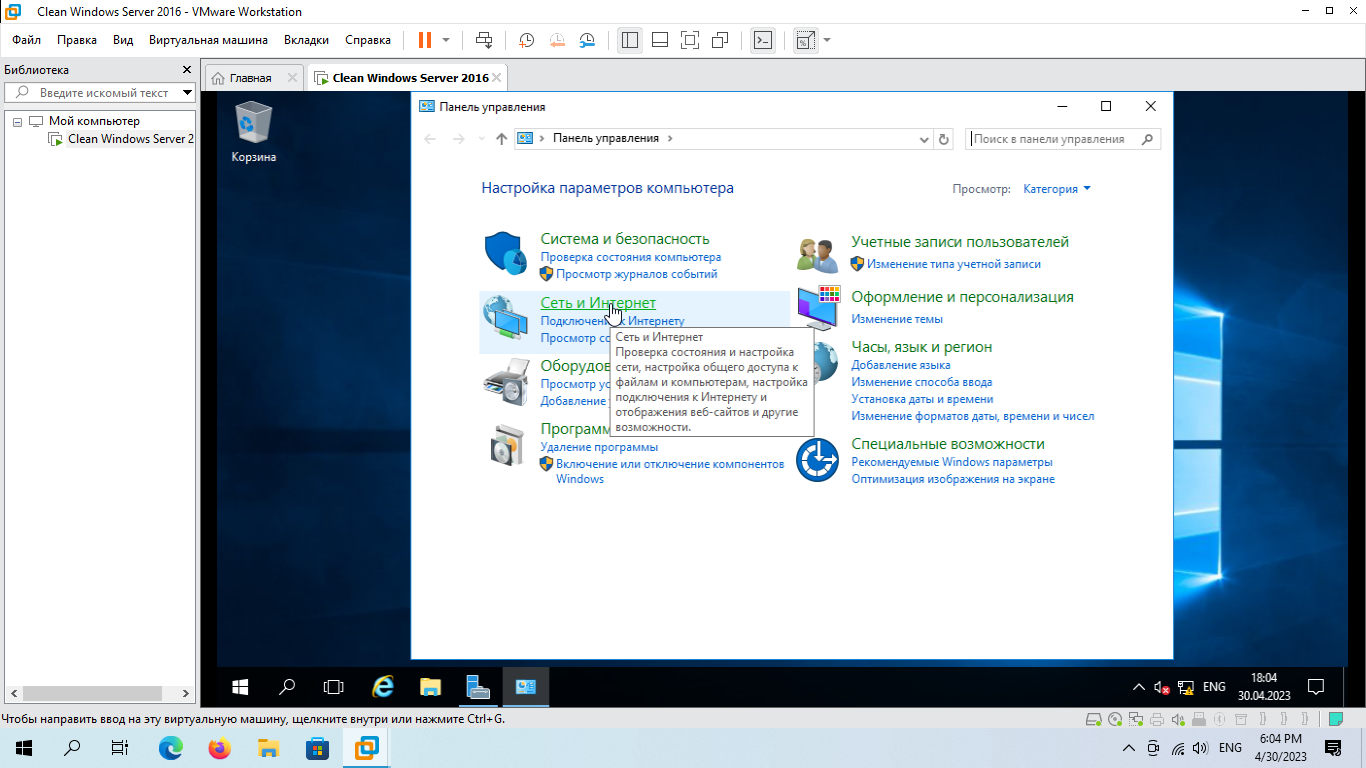
\includegraphics[width=0.85\textwidth]{Screenshot_19}
    \caption{Переходим в пункт "Сеть и Интернет"}
    \label{img:19}
  \end{figure}

  \begin{figure}[H]
    \centering
    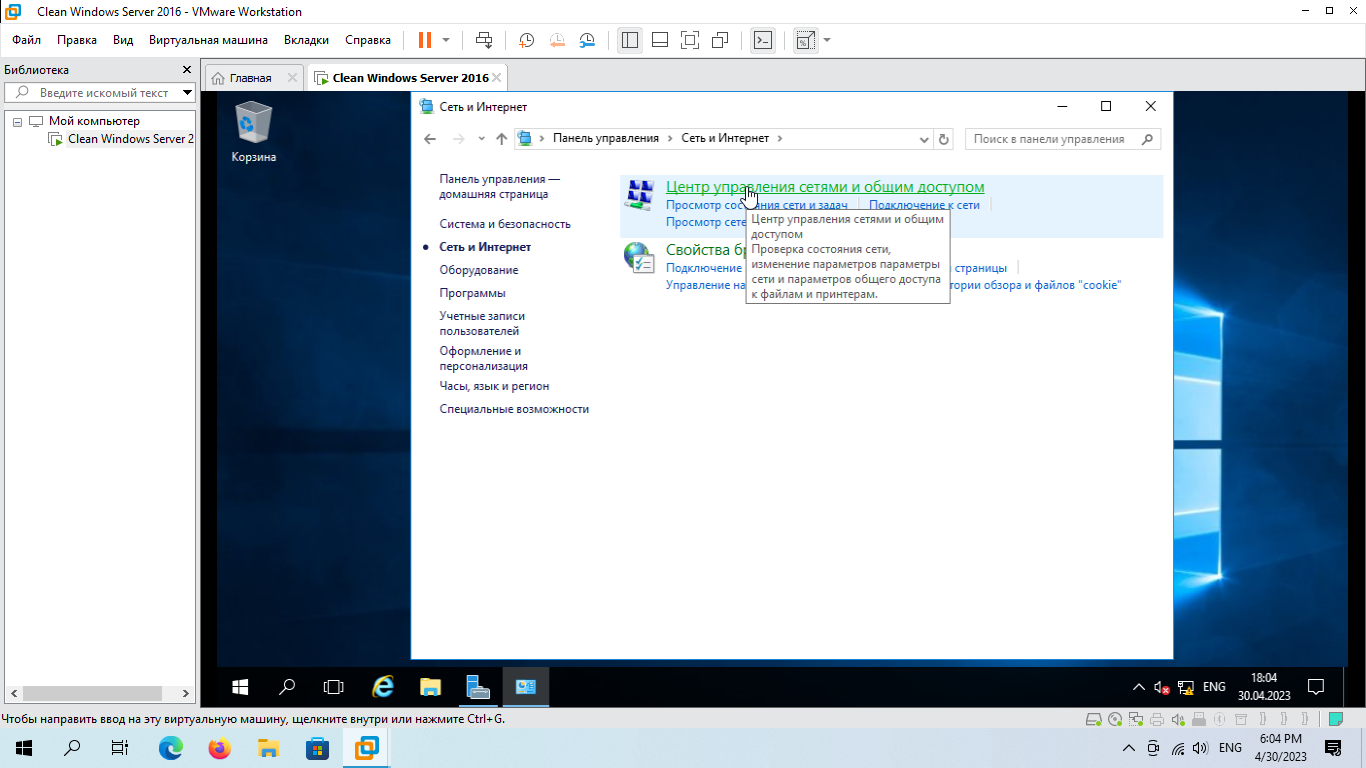
\includegraphics[width=0.85\textwidth]{Screenshot_20}
    \caption{Заходим в центр управления сетями и общим доступом}
    \label{img:20}
  \end{figure}

  \begin{figure}[H]
    \centering
    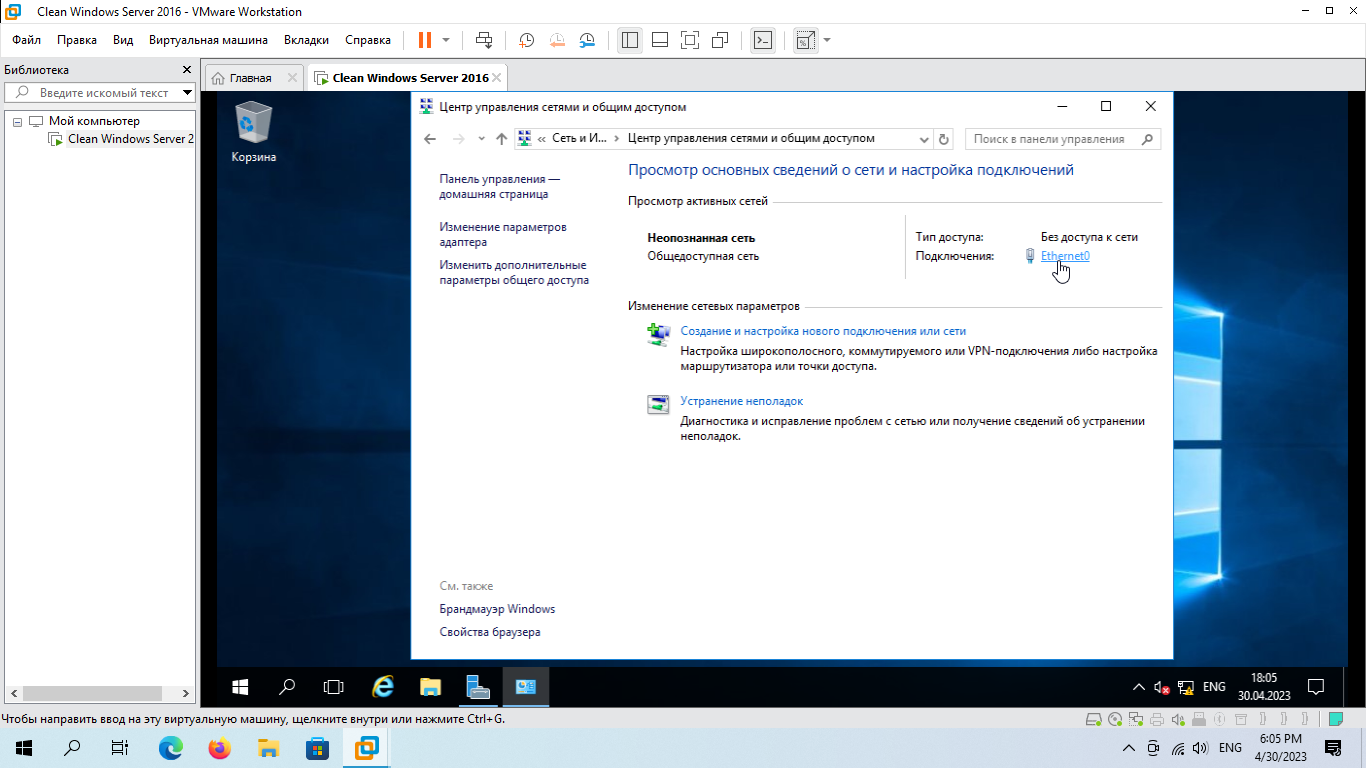
\includegraphics[width=0.85\textwidth]{Screenshot_22}
    \caption{Выбираем необходимый сетевой адаптер - \textit{Ethernet}}
    \label{img:22}
  \end{figure}

  \begin{figure}[H]
    \centering
    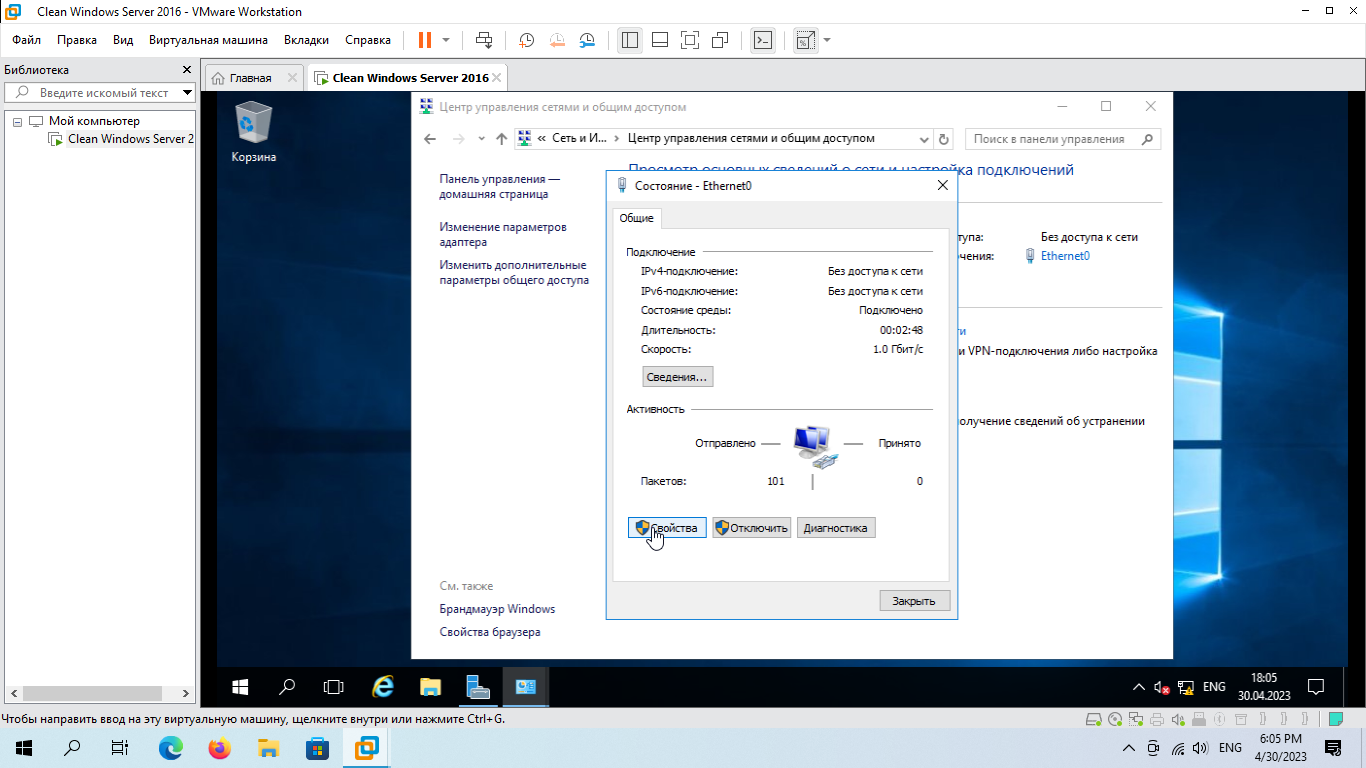
\includegraphics[width=0.85\textwidth]{Screenshot_24}
    \caption{Открываем его свойства}
    \label{img:24}
  \end{figure}

  \begin{figure}[H]
    \centering
    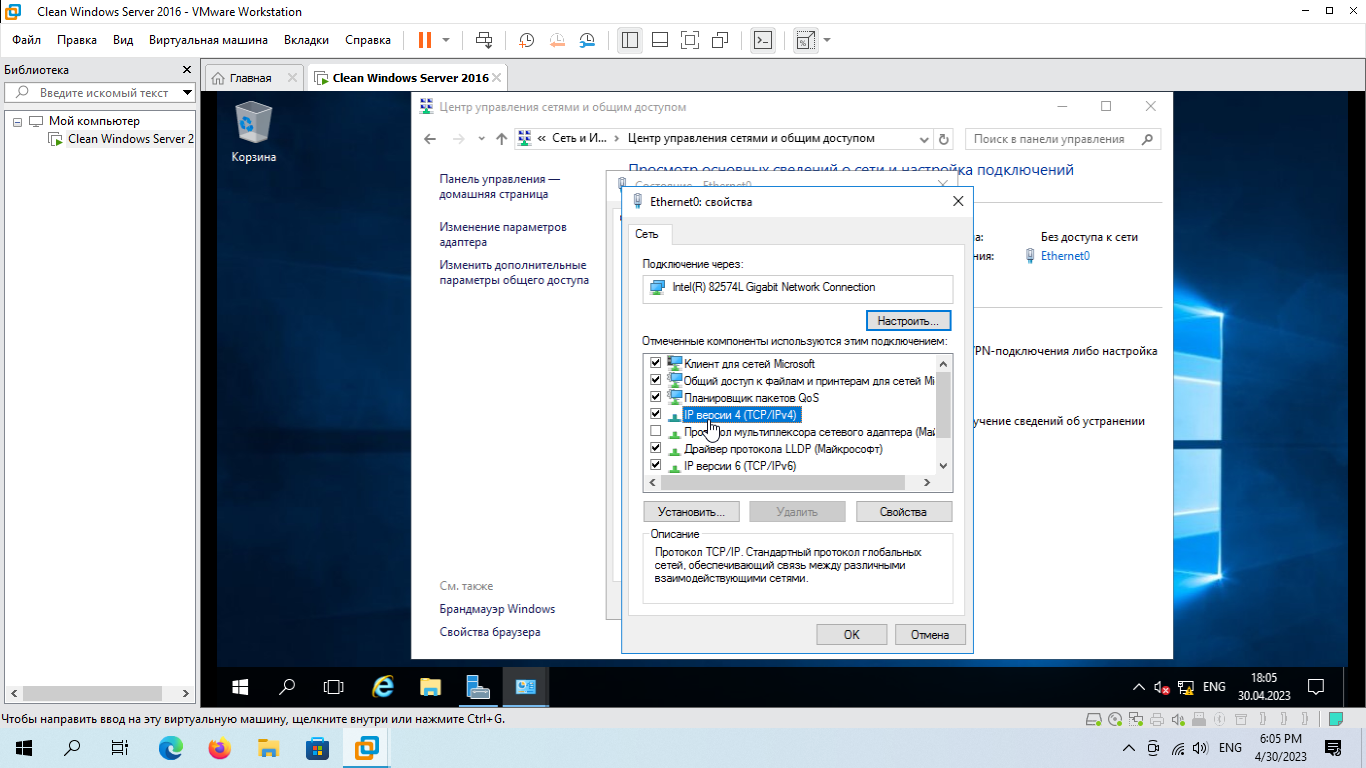
\includegraphics[width=0.85\textwidth]{Screenshot_25}
    \caption{Заходим в параметры \textit{IPv4}}
    \label{img:25}
  \end{figure}

  \begin{figure}[H]
    \centering
    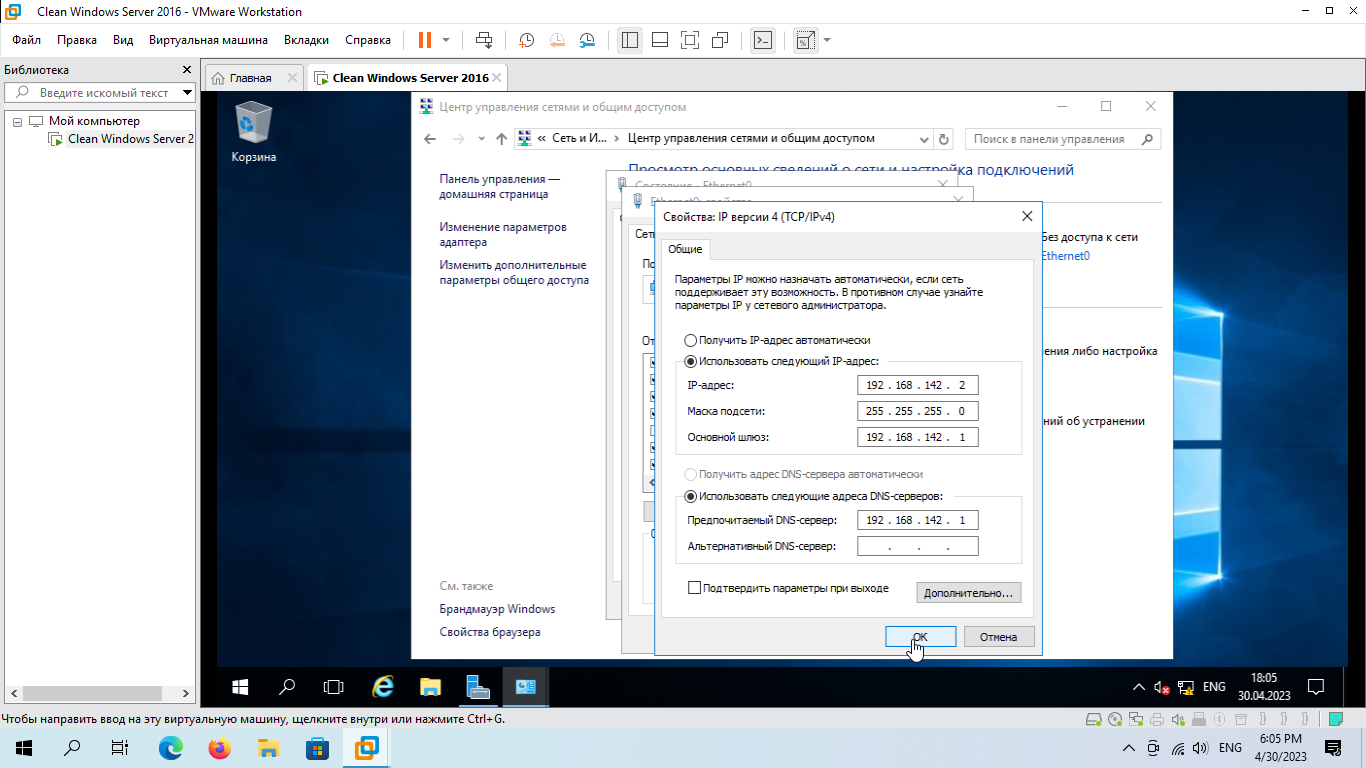
\includegraphics[width=0.85\textwidth]{Screenshot_26}
    \caption{Выполняем необходимые настройки}
    \label{img:26}
  \end{figure}

  В качестве \textit{IP} адреса был выбран первый свободный - 192.168.142.2 (192.168.142.0 - адрес сети, уже занят, и
  192.168.142.1 - адрес шлюза, тоже занят). Также указываем маску, адрес шлюза и \textit{DNS} (такой же, как шлюз).

  \begin{figure}[H]
    \centering
    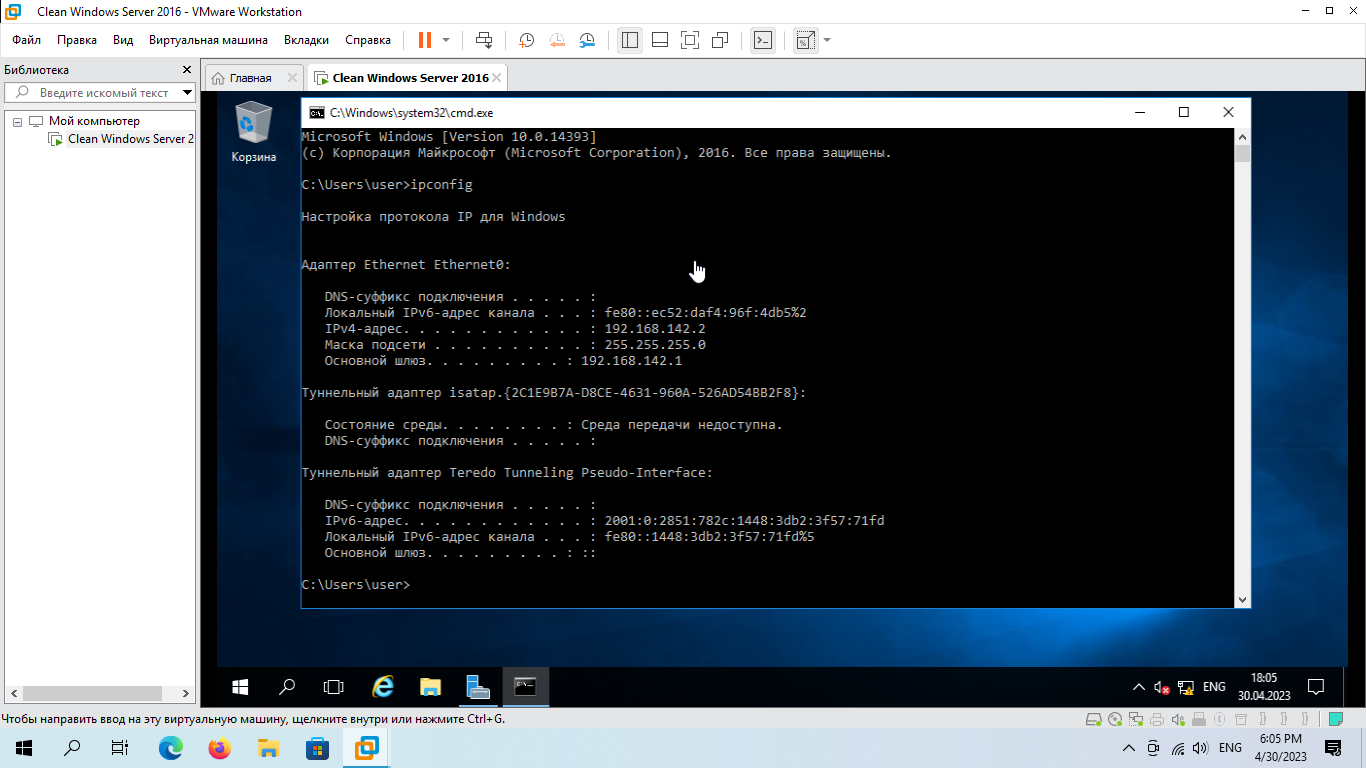
\includegraphics[width=0.85\textwidth]{Screenshot_27}
    \caption{Проверим новую конфигурацию при помощи \textit{ipconfig}}
    \label{img:27}
  \end{figure}

  Теперь нужно удостовериться, что машина может достучаться до шлюза, имеет доступ в Интернет
  и может делать \textit{DNS} запросы:

  \begin{figure}[H]
    \centering
    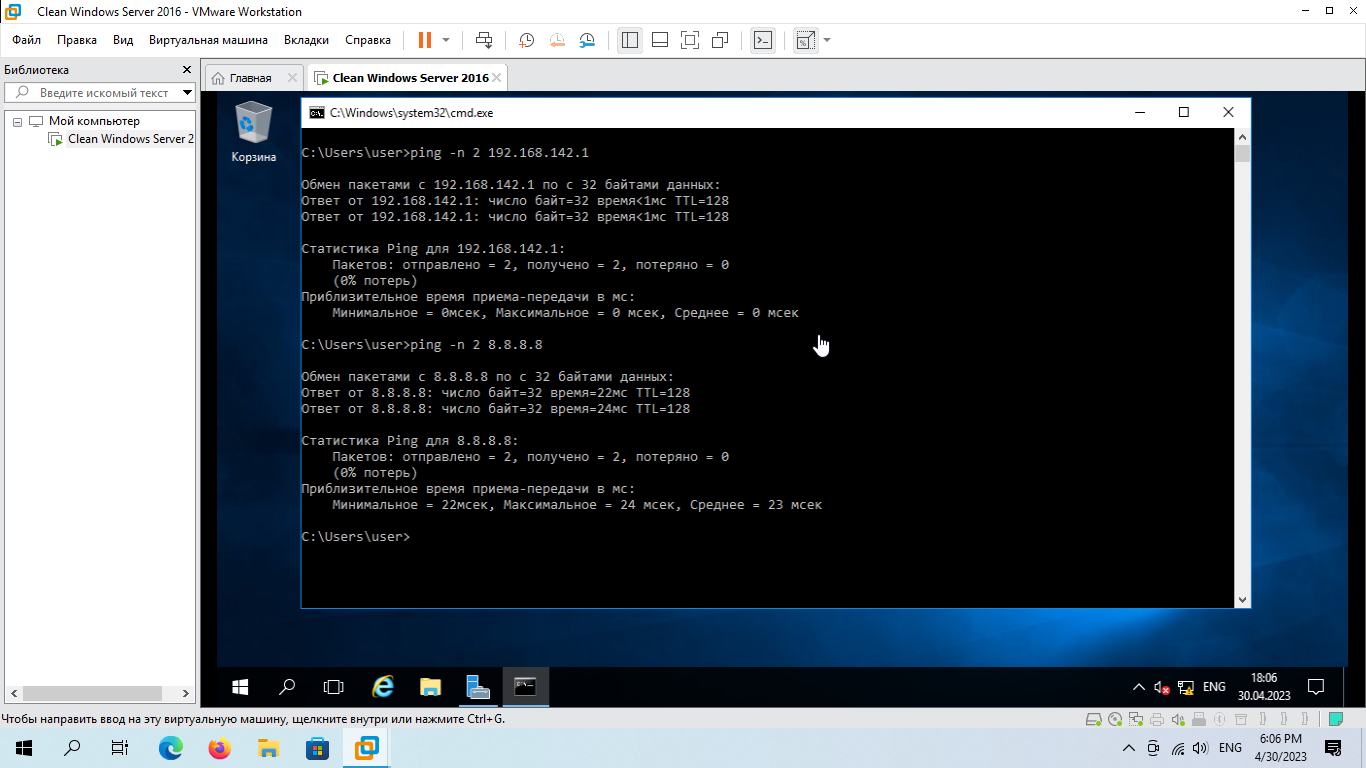
\includegraphics[width=0.85\textwidth]{Screenshot_29}
    \caption{Пинг шлюза и google dns - доступ в сеть есть}
    \label{img:29}
  \end{figure}

  \begin{figure}[H]
    \centering
    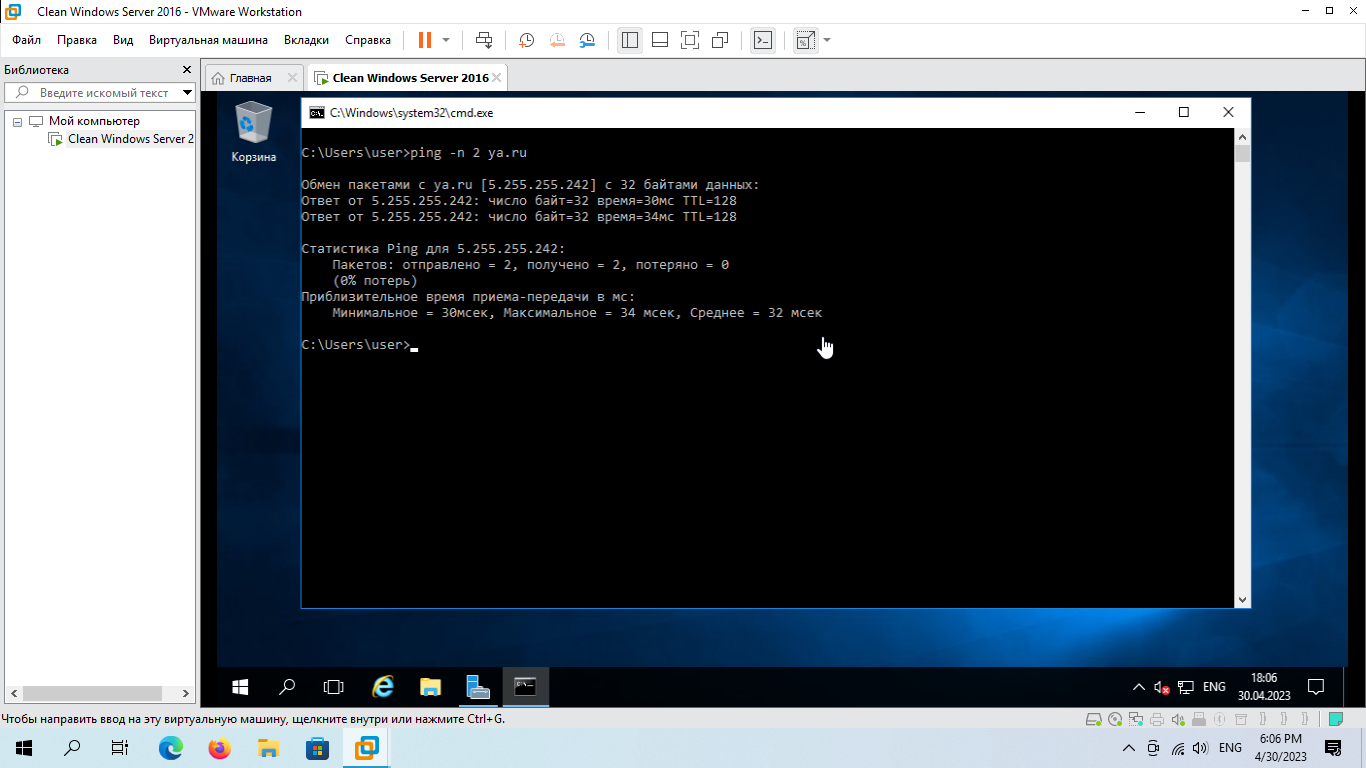
\includegraphics[width=0.85\textwidth]{Screenshot_30}
    \caption{Пинг ya.ru - \textit{DNS} работает}
    \label{img:30}
  \end{figure}

  \subsubsection{Настройка пароля администратора}

  Необходимо задать пароль для доступа к учетной записи администратора:

  \begin{figure}[H]
    \centering
    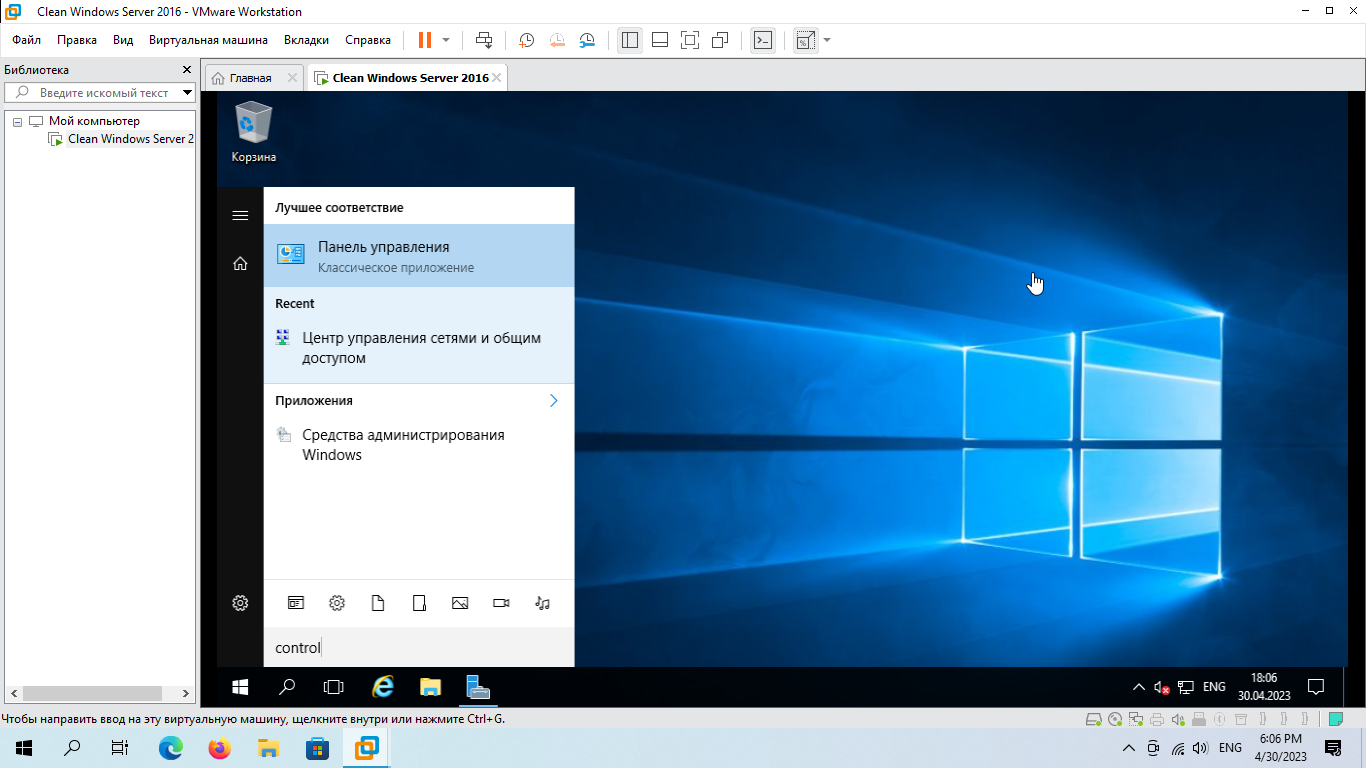
\includegraphics[width=0.85\textwidth]{Screenshot_31}
    \caption{Открываем Панель Управления}
    \label{img:31}
  \end{figure}

  \begin{figure}[H]
    \centering
    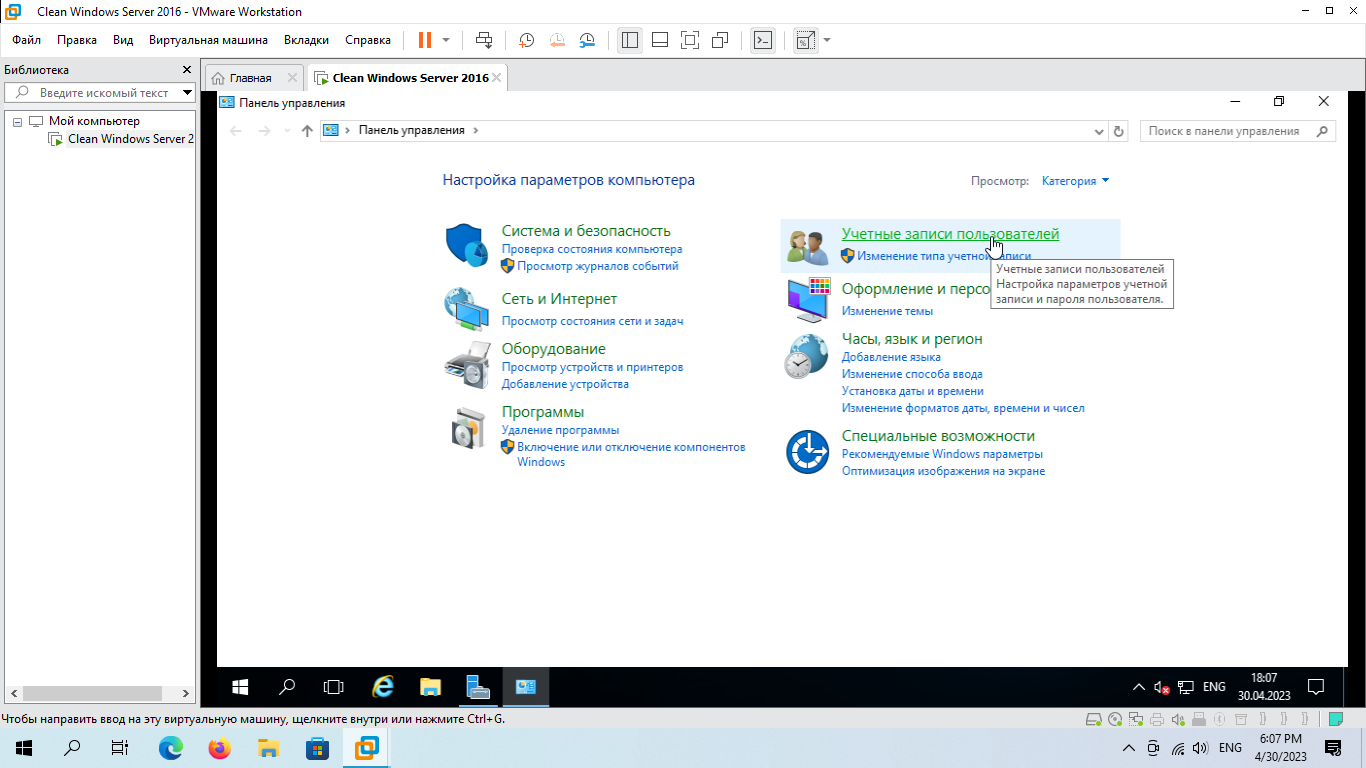
\includegraphics[width=0.85\textwidth]{Screenshot_32}
    \caption{Заходим в пункт "Учетные записи пользователей"}
    \label{img:32}
  \end{figure}

  \begin{figure}[H]
    \centering
    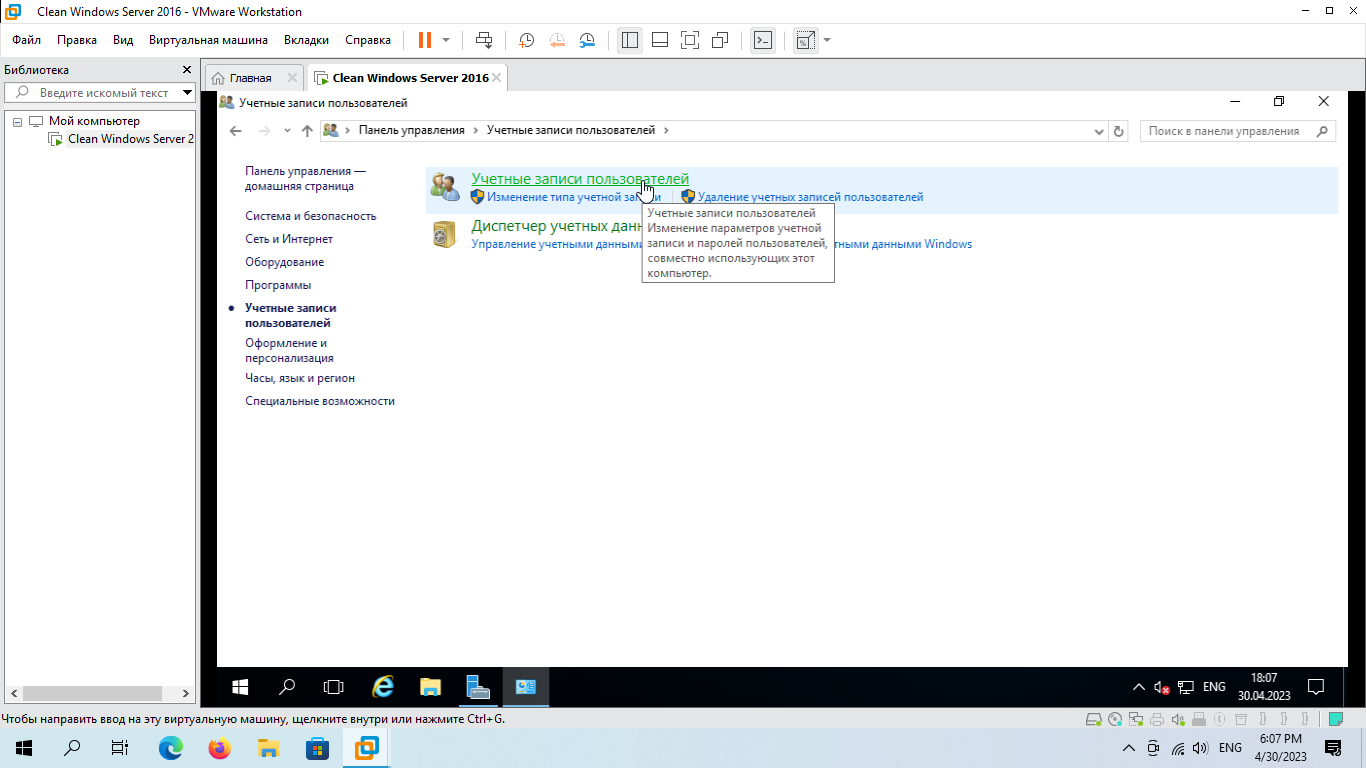
\includegraphics[width=0.85\textwidth]{Screenshot_33}
    \caption{Учетные записи пользователей}
    \label{img:33}
  \end{figure}

  \begin{figure}[H]
    \centering
    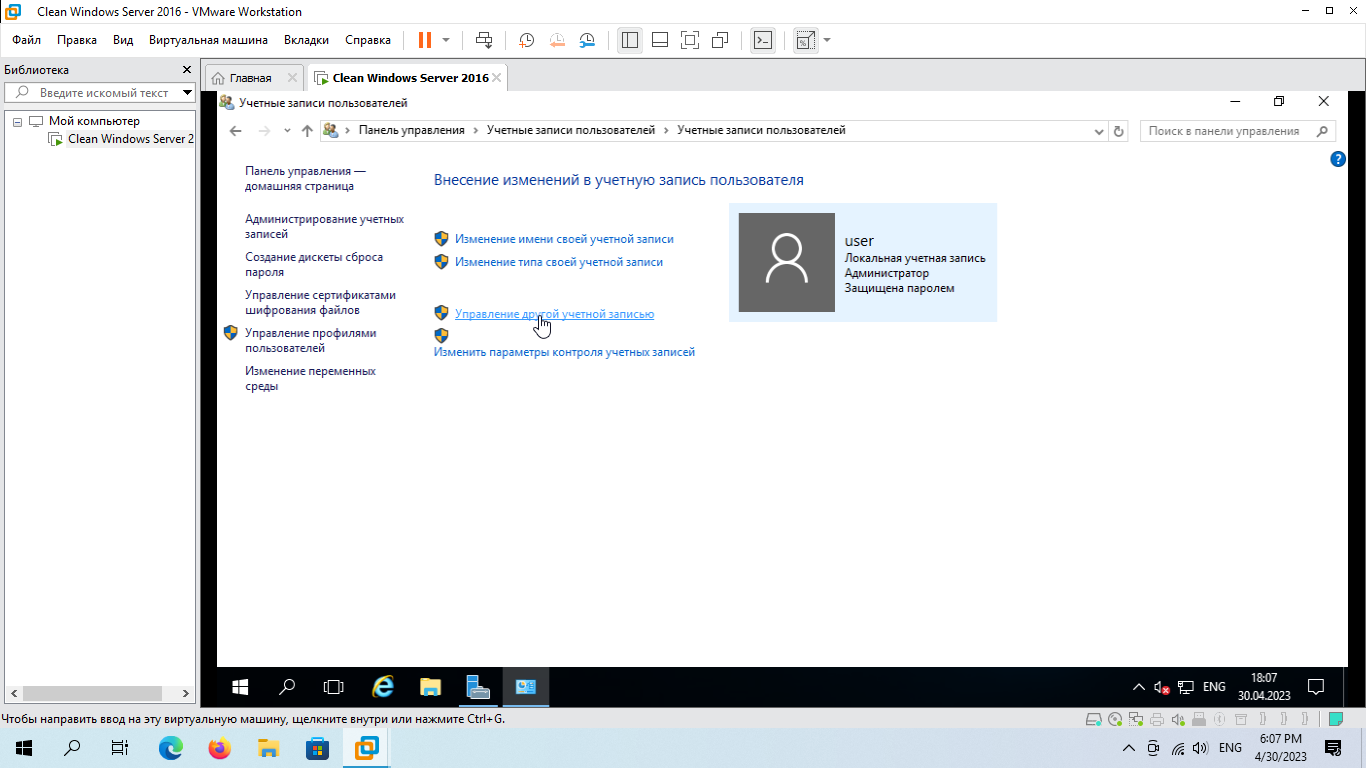
\includegraphics[width=0.85\textwidth]{Screenshot_34}
    \caption{Настроить нужно не учетную запись текущего пользователя - "Управление другой учетной записью"}
    \label{img:34}
  \end{figure}

  \begin{figure}[H]
    \centering
    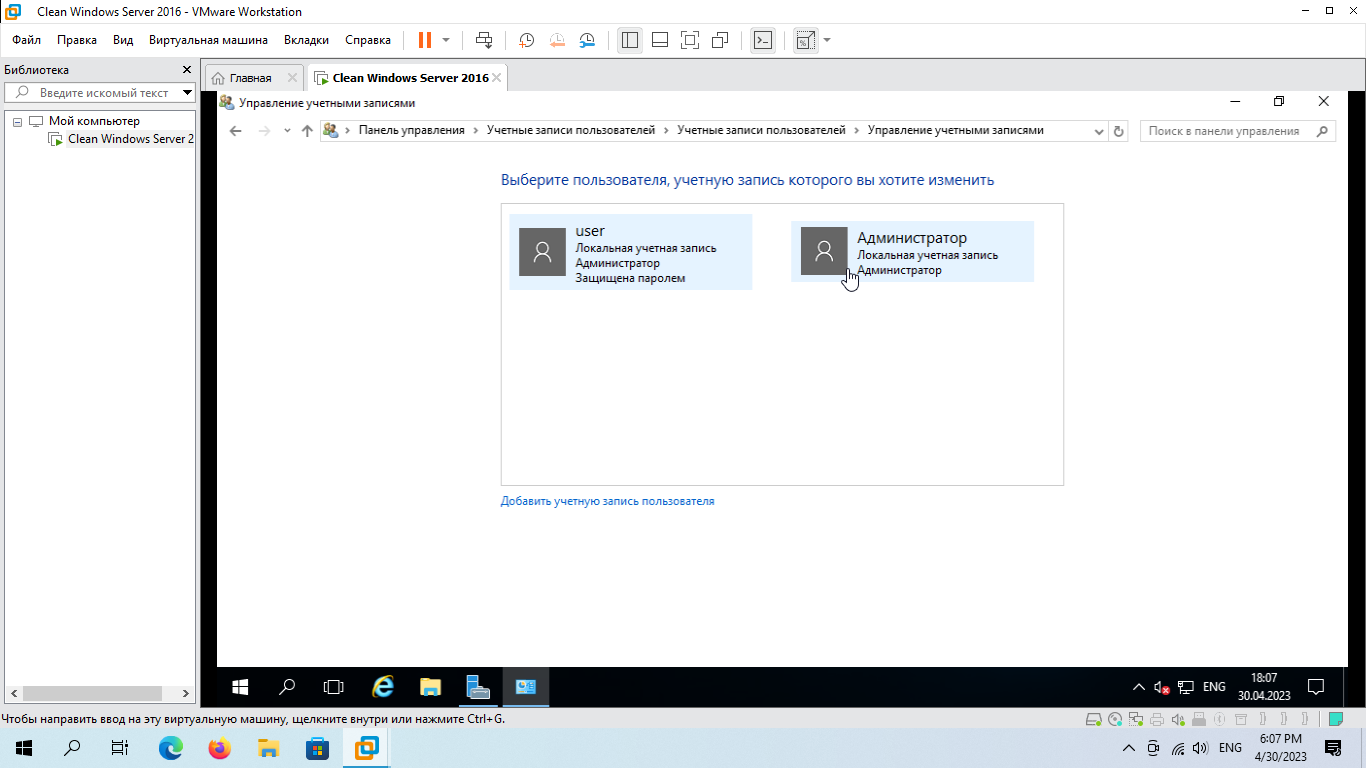
\includegraphics[width=0.85\textwidth]{Screenshot_35}
    \caption{Выбираем Администратора}
    \label{img:35}
  \end{figure}

  \begin{figure}[H]
    \centering
    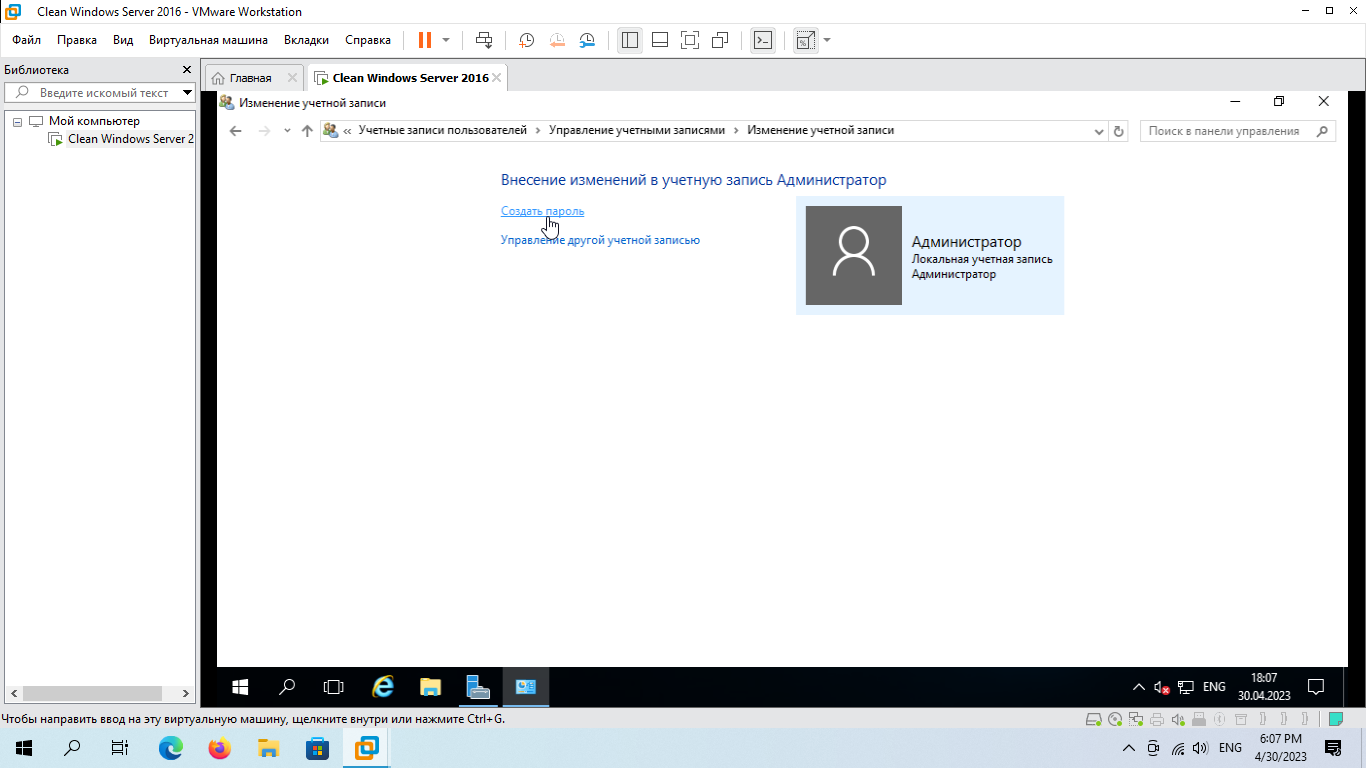
\includegraphics[width=0.85\textwidth]{Screenshot_36}
    \caption{Нажимаем "Создать пароль"}
    \label{img:36}
  \end{figure}

  \begin{figure}[H]
    \centering
    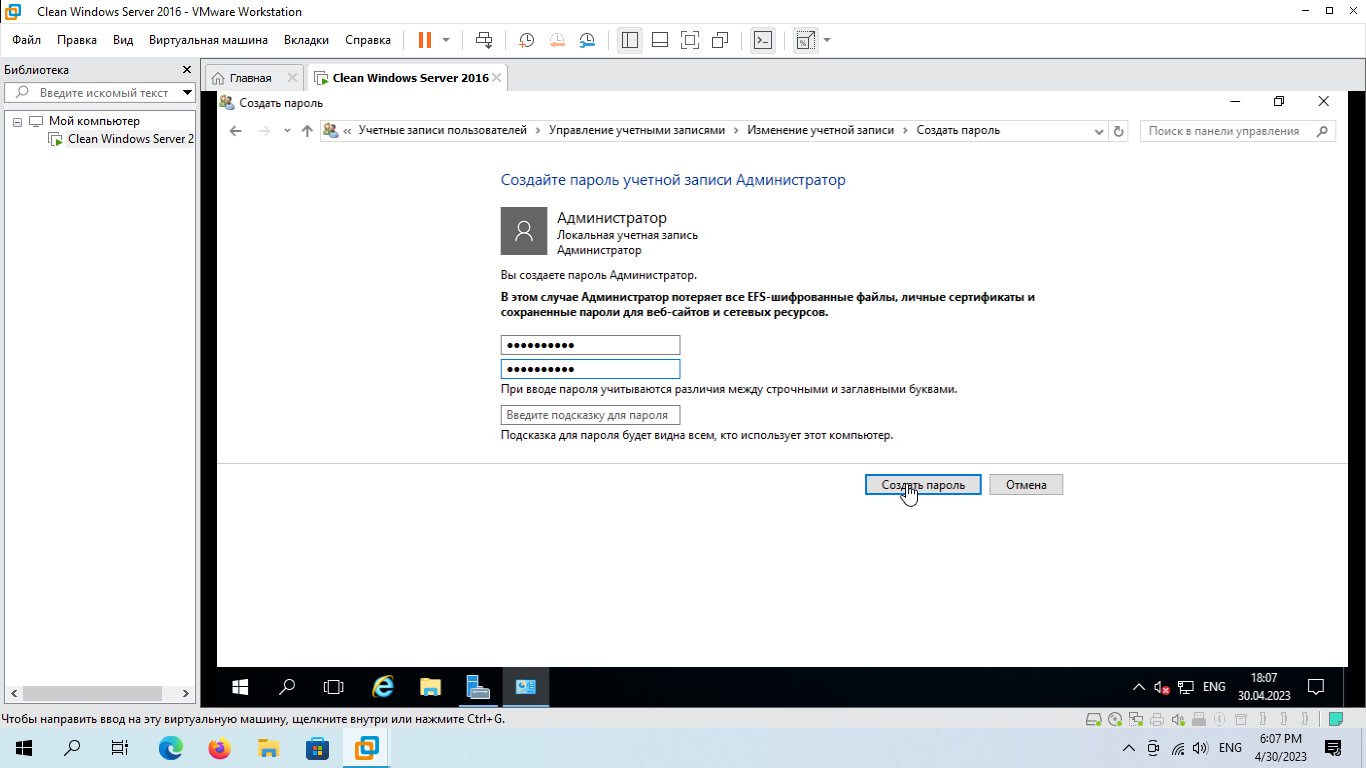
\includegraphics[width=0.85\textwidth]{Screenshot_37}
    \caption{Указываем новый пароль}
    \label{img:37}
  \end{figure}

  Готово - теперь для доступа к правам Администратора необходимо знать пароль.

  \subsubsection{Настройка домена}

  Теперь настроим домен и создадим новых пользователей:

  \begin{figure}[H]
    \centering
    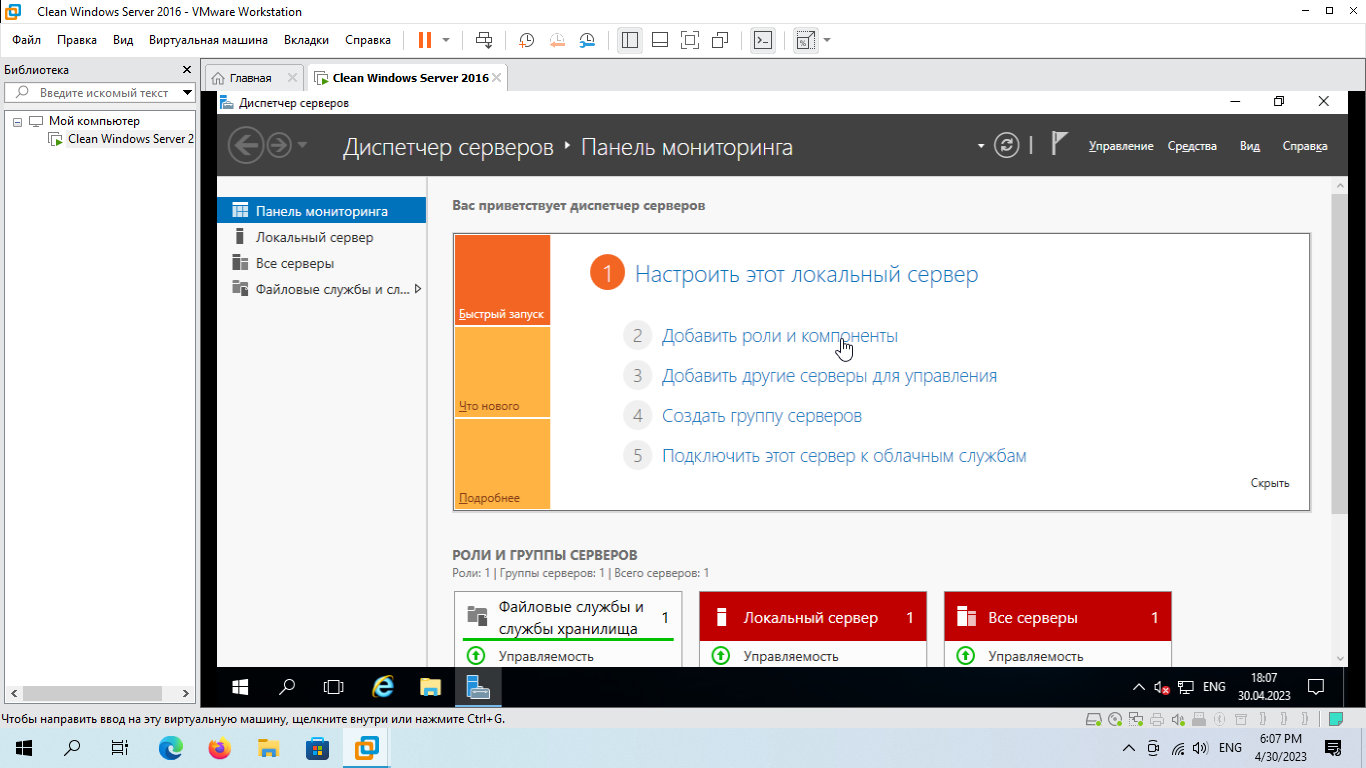
\includegraphics[width=0.85\textwidth]{Screenshot_38}
    \caption{Открываем диспетчер серверов и начинаем добавление ролей и компонентов}
    \label{img:38}
  \end{figure}

  \begin{figure}[H]
    \centering
    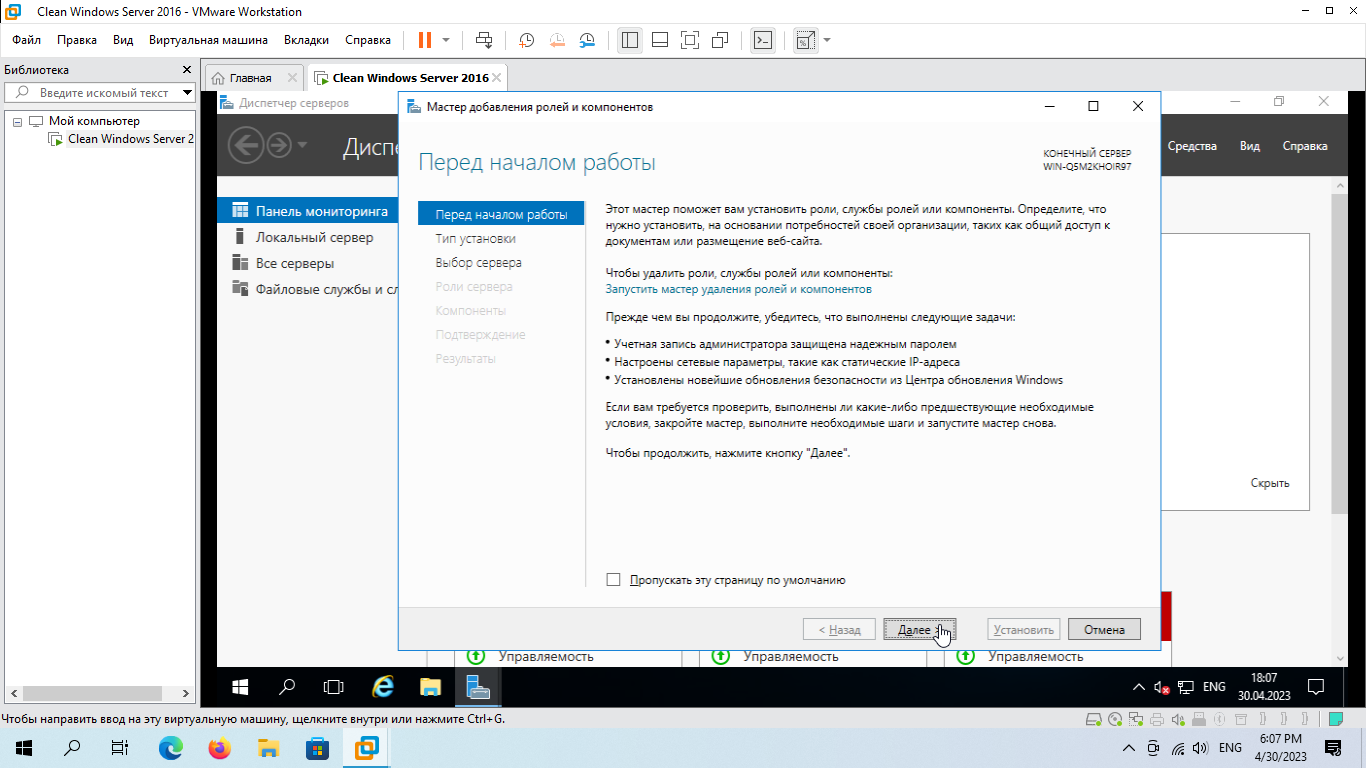
\includegraphics[width=0.85\textwidth]{Screenshot_39}
    \caption{Далее}
    \label{img:39}
  \end{figure}

  \begin{figure}[H]
    \centering
    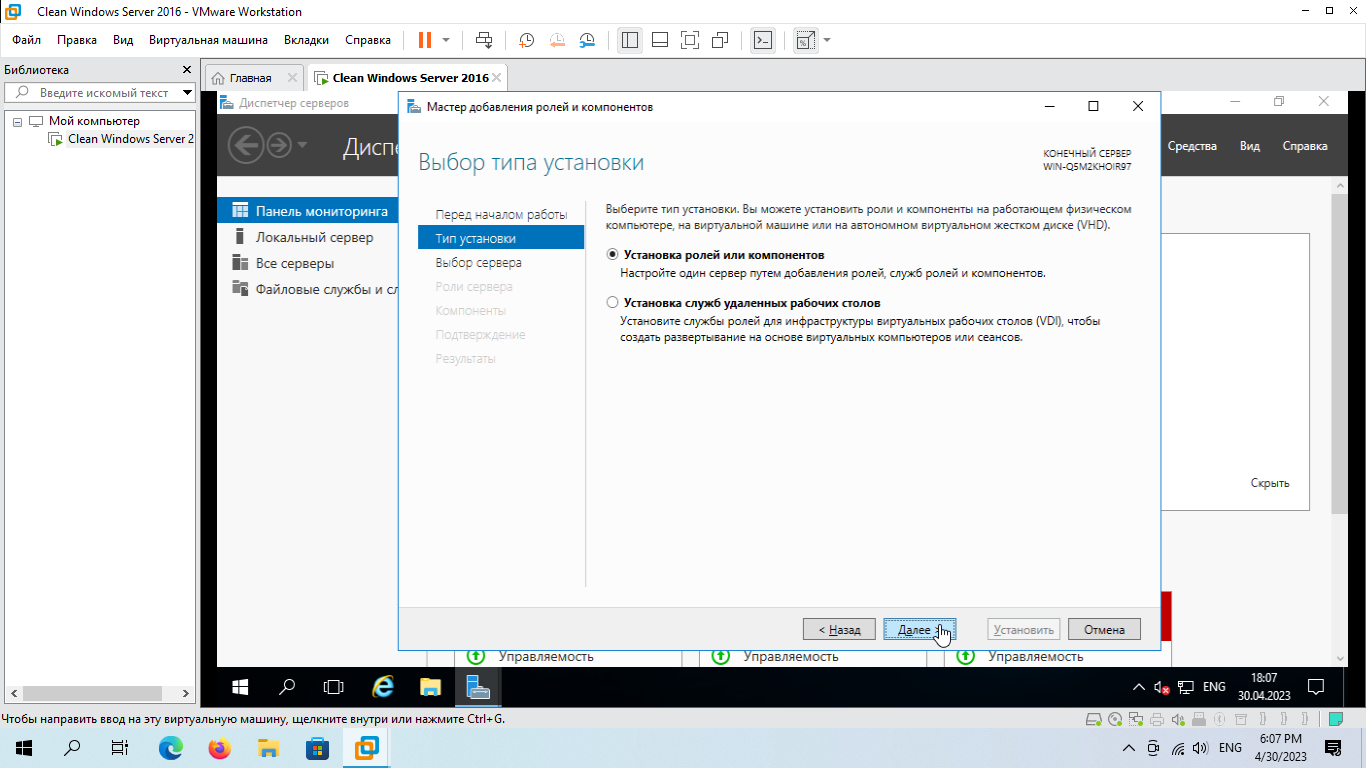
\includegraphics[width=0.85\textwidth]{Screenshot_40}
    \caption{Выбираем тип установки - нам нужны новые роли и компоненты}
    \label{img:40}
  \end{figure}

  \begin{figure}[H]
    \centering
    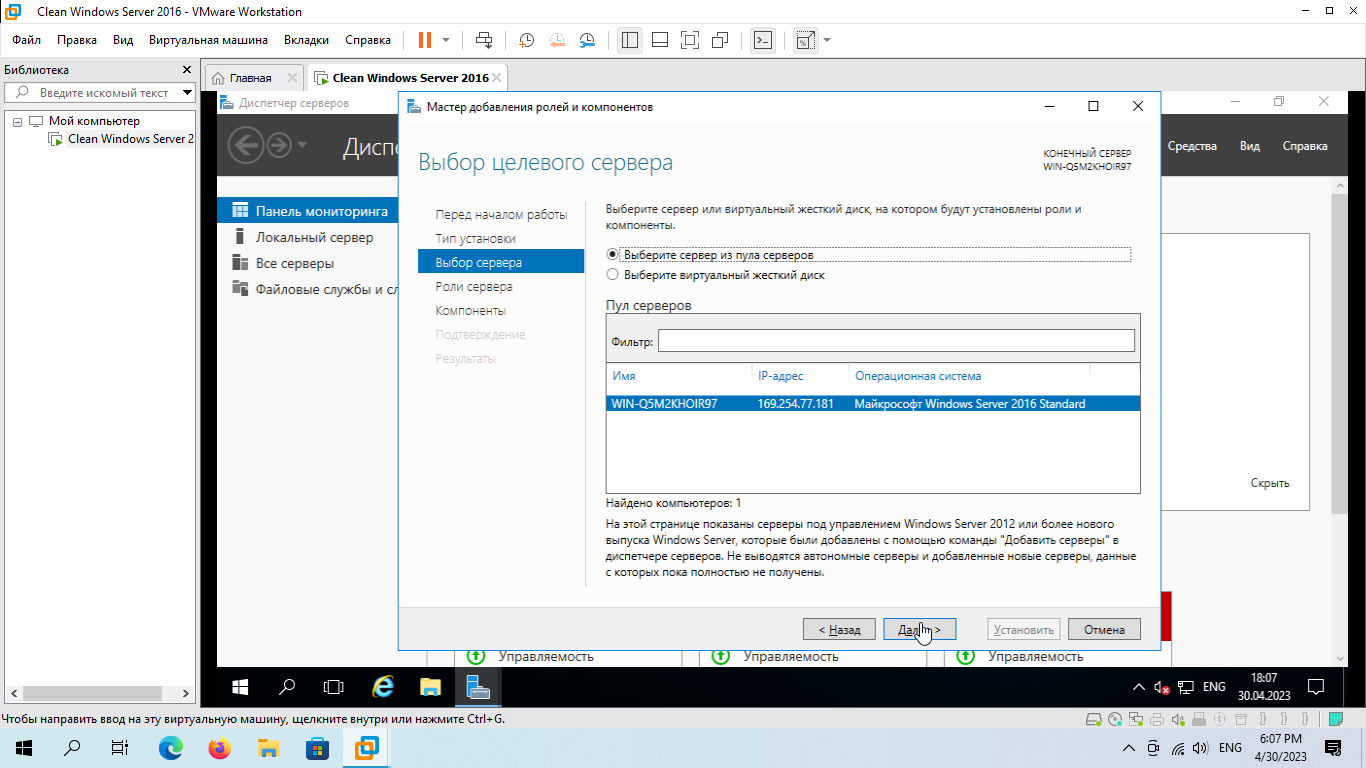
\includegraphics[width=0.85\textwidth]{Screenshot_41}
    \caption{Устанавливаем все для текущего сервера}
    \label{img:41}
  \end{figure}

  \begin{figure}[H]
    \centering
    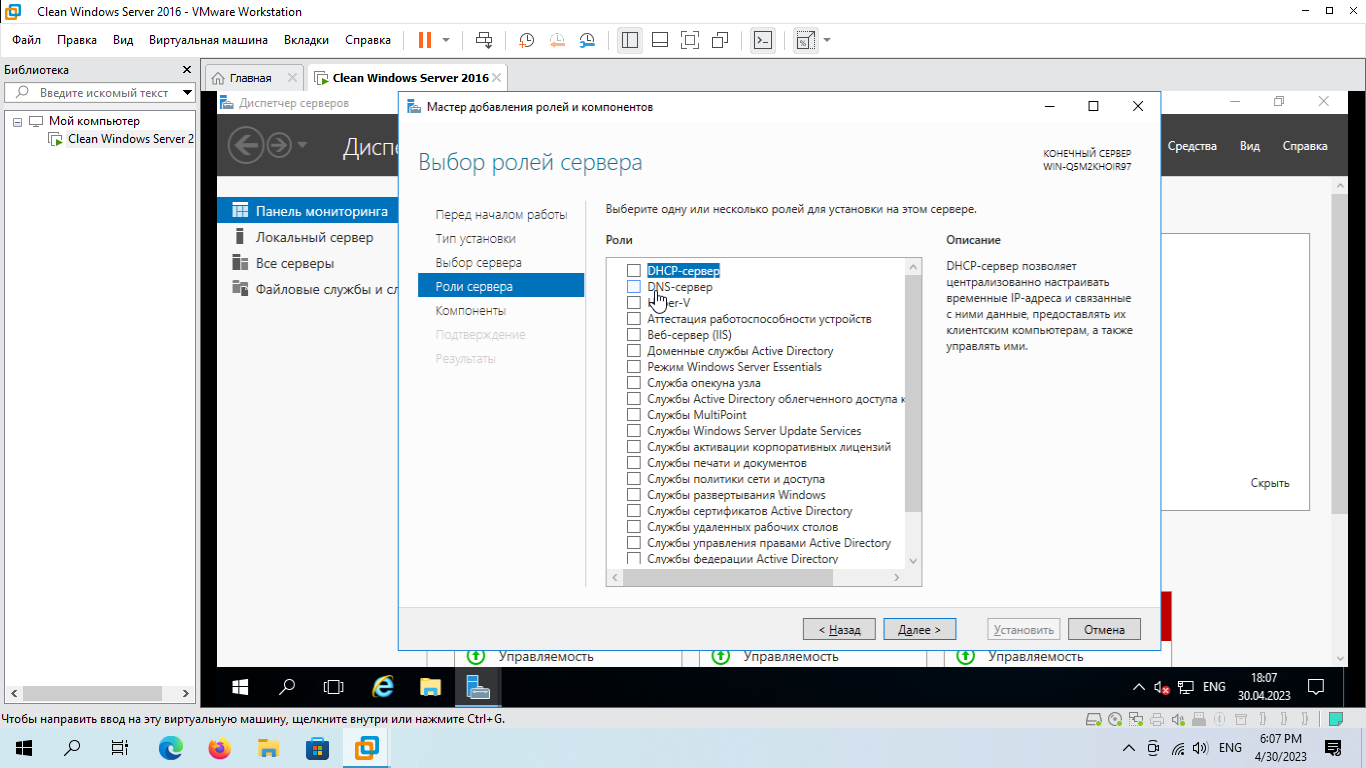
\includegraphics[width=0.85\textwidth]{Screenshot_42}
    \caption{Добавляем новую роль - \textit{DNS}-сервер}
    \label{img:42}
  \end{figure}

  \begin{figure}[H]
    \centering
    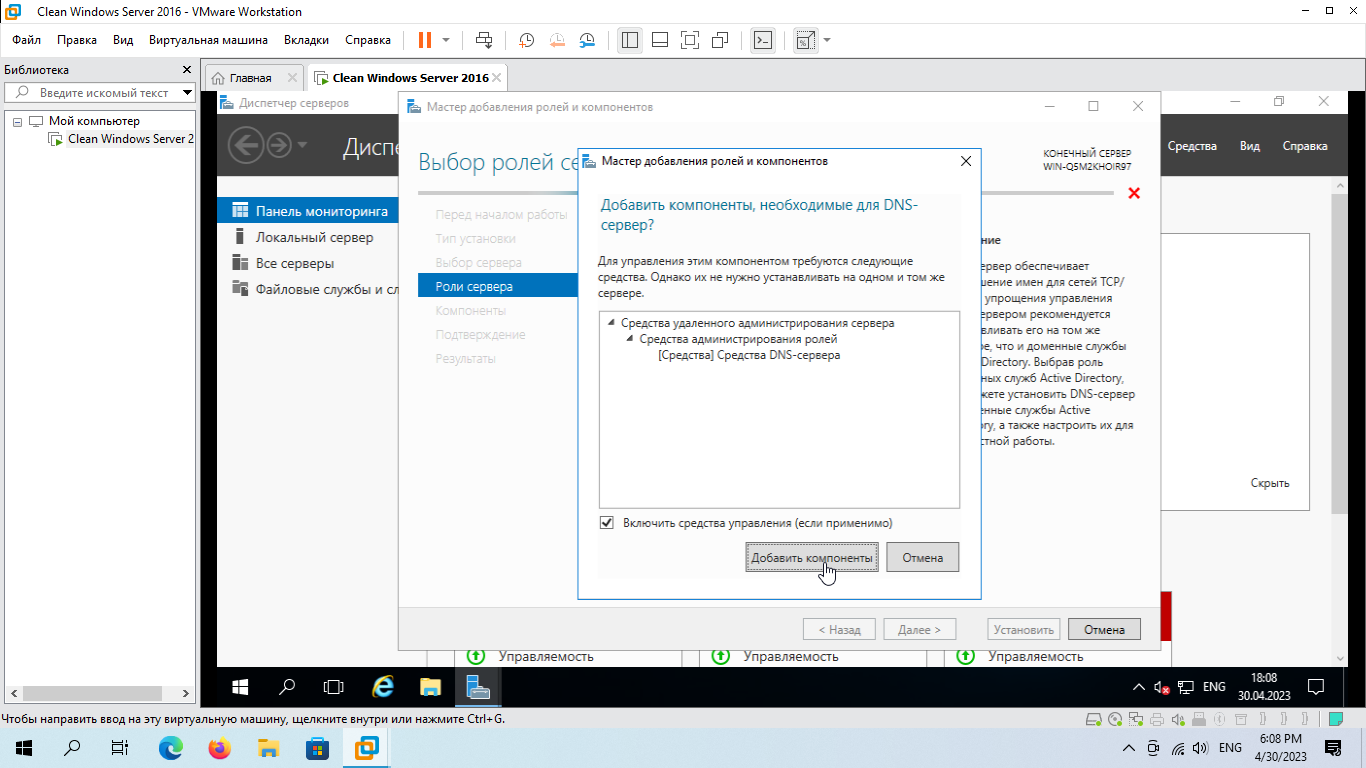
\includegraphics[width=0.85\textwidth]{Screenshot_43}
    \caption{Добавляем компонент, необходимые для новой роли}
    \label{img:43}
  \end{figure}

  \begin{figure}[H]
    \centering
    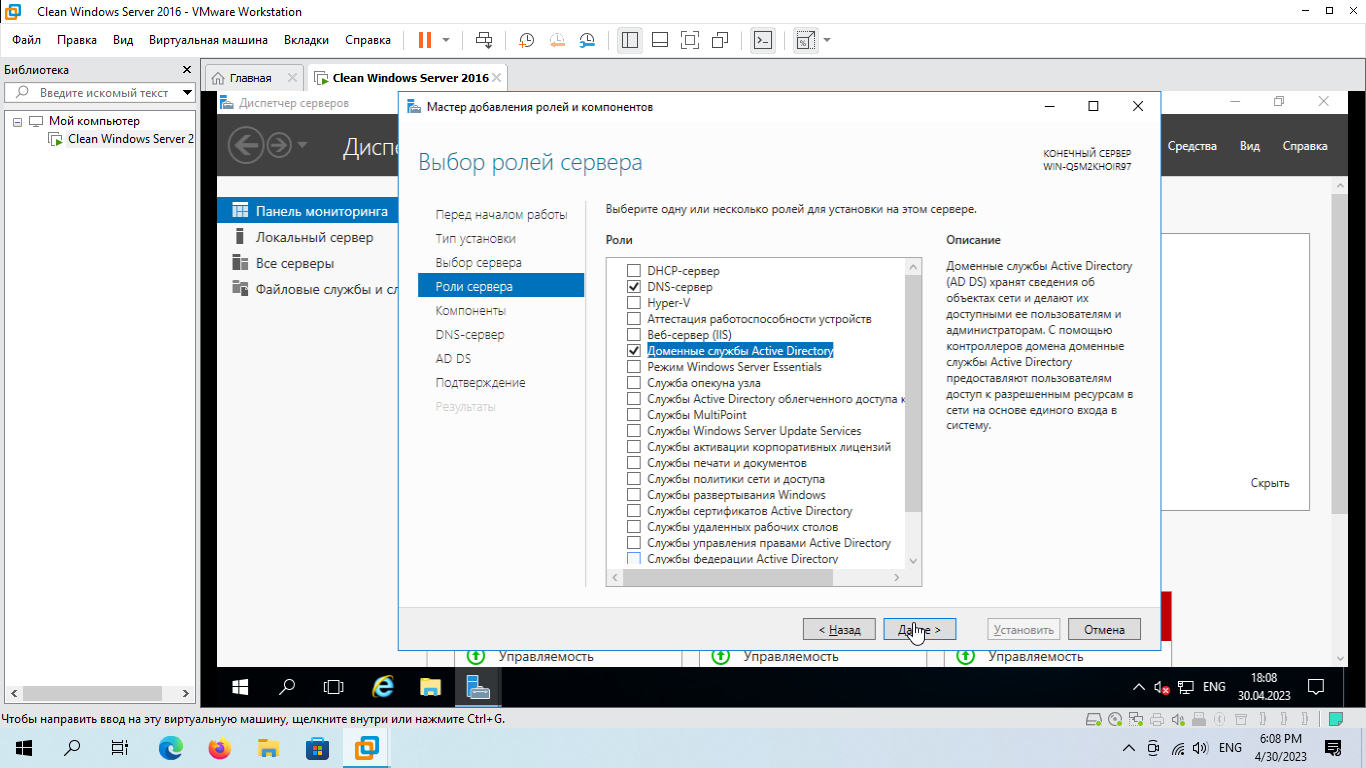
\includegraphics[width=0.85\textwidth]{Screenshot_44}
    \caption{Также необходимо добавить роль "Доменные службы Active Directory"}
    \label{img:44}
  \end{figure}

  \begin{figure}[H]
    \centering
    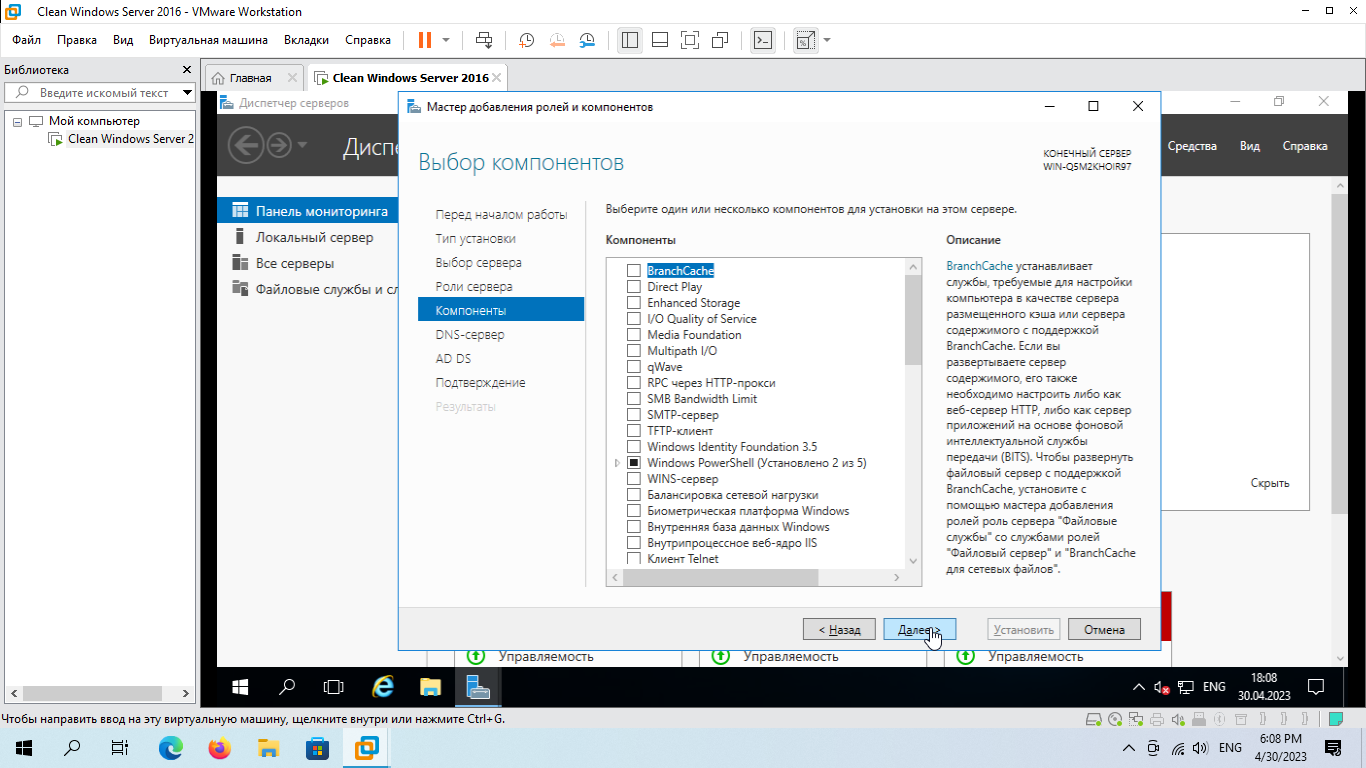
\includegraphics[width=0.85\textwidth]{Screenshot_45}
    \caption{Дополнительные компоненты не нужны}
    \label{img:45}
  \end{figure}

  \begin{figure}[H]
    \centering
    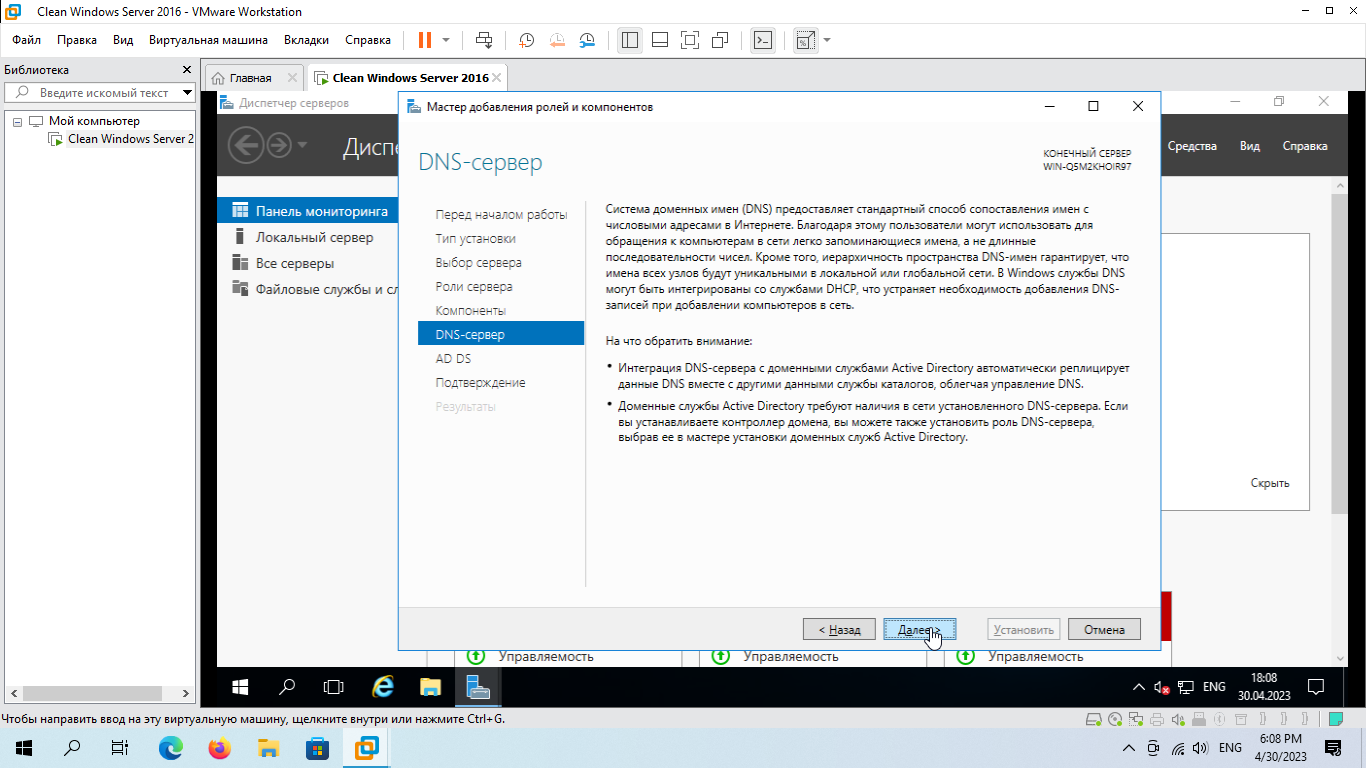
\includegraphics[width=0.85\textwidth]{Screenshot_46}
    \caption{Соглашаемся}
    \label{img:46}
  \end{figure}

  \begin{figure}[H]
    \centering
    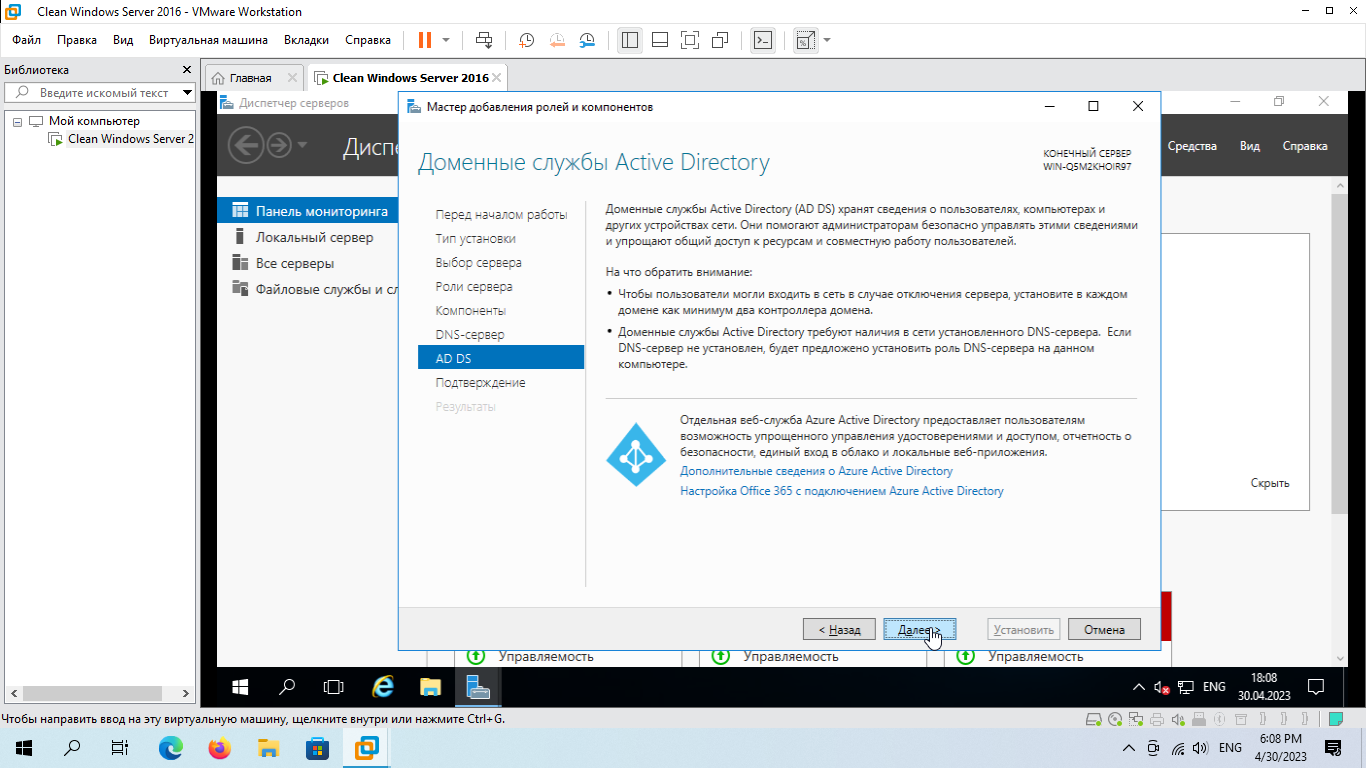
\includegraphics[width=0.85\textwidth]{Screenshot_47}
    \caption{Также соглашаемся}
    \label{img:47}
  \end{figure}

  \begin{figure}[H]
    \centering
    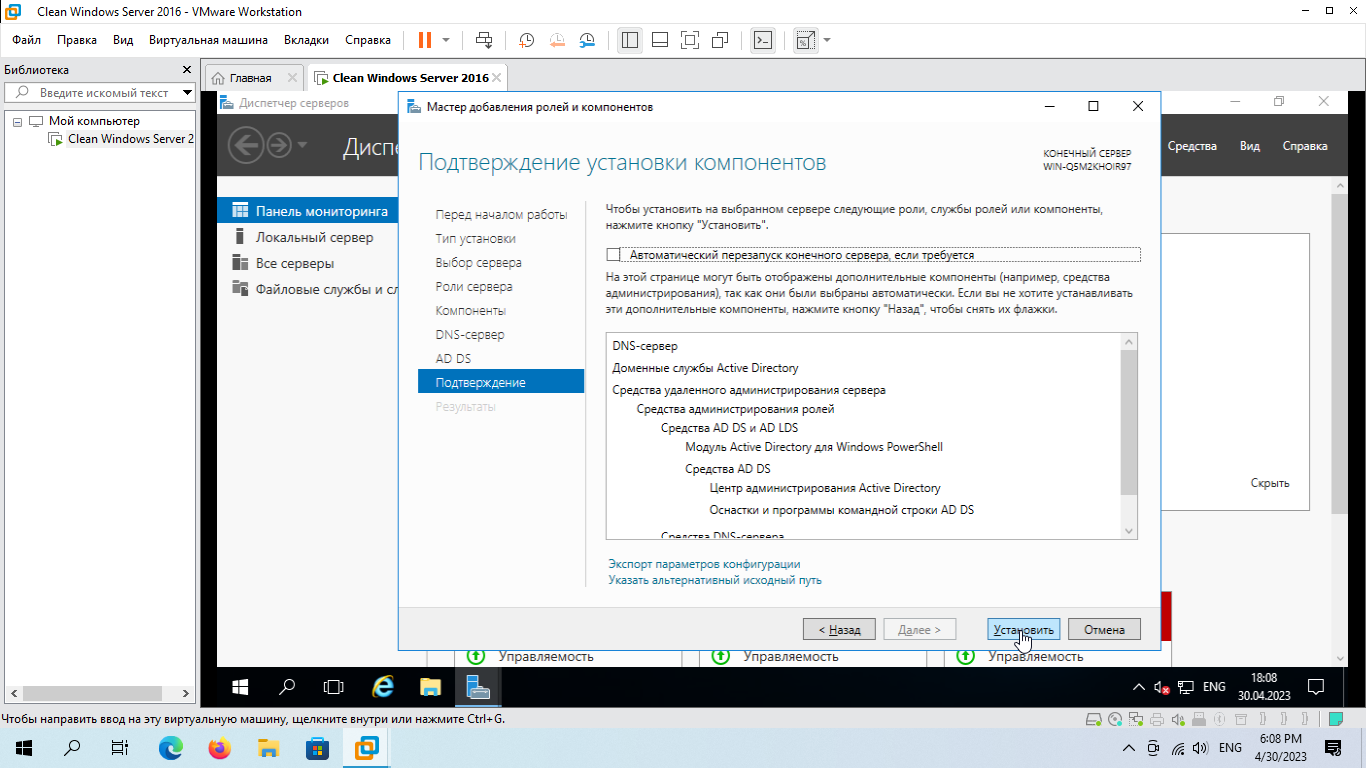
\includegraphics[width=0.85\textwidth]{Screenshot_48}
    \caption{Начинаем установку необходимых ролей}
    \label{img:48}
  \end{figure}

  \begin{figure}[H]
    \centering
    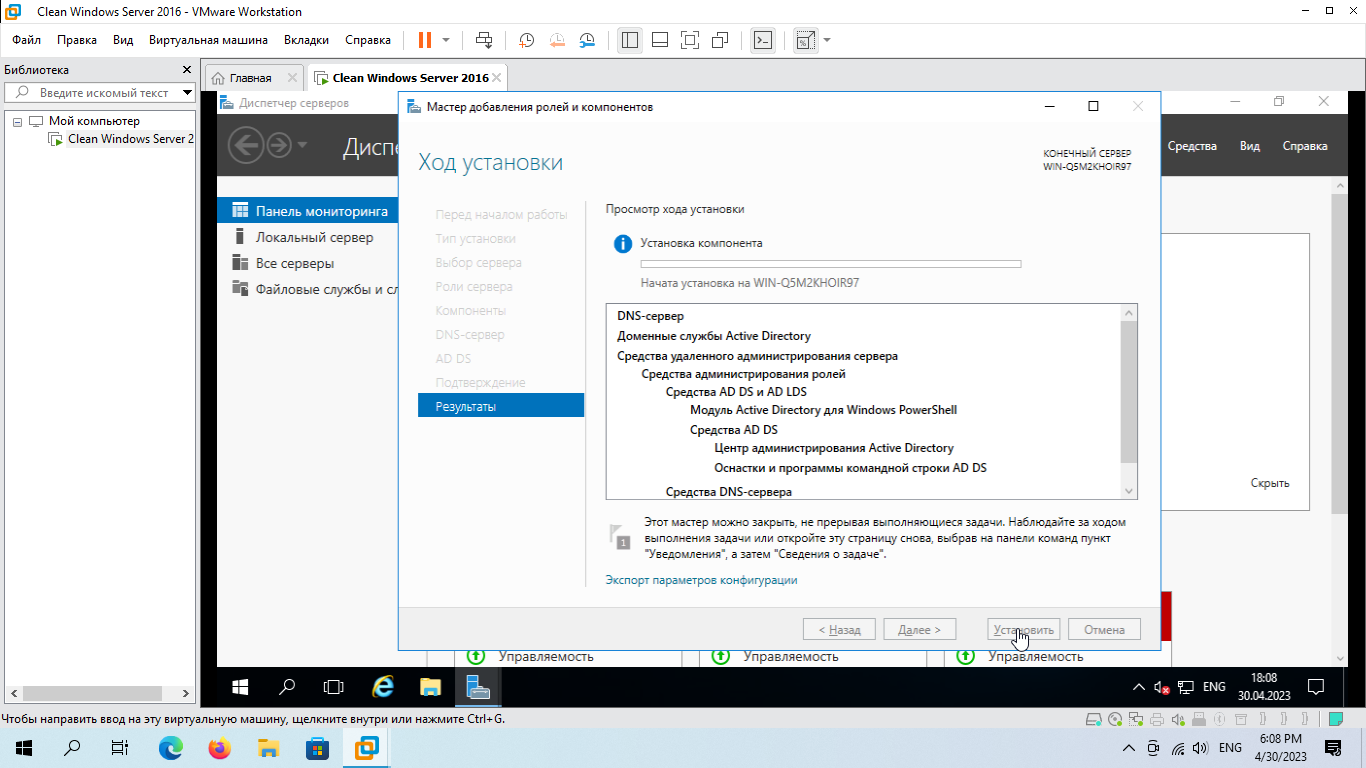
\includegraphics[width=0.85\textwidth]{Screenshot_49}
    \caption{Ждем}
    \label{img:49}
  \end{figure}

  \begin{figure}[H]
    \centering
    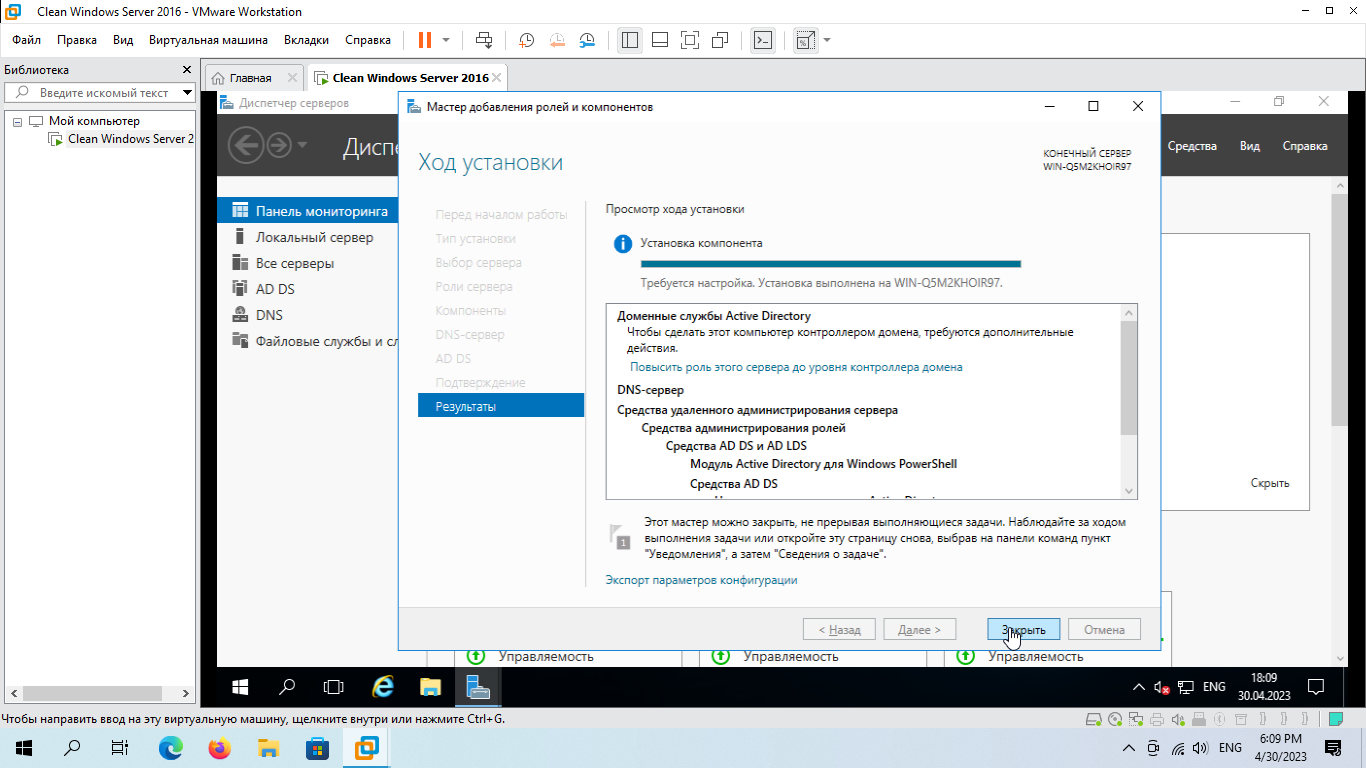
\includegraphics[width=0.85\textwidth]{Screenshot_50}
    \caption{Все необходимое установлено}
    \label{img:50}
  \end{figure}

  Далее необходимо повысить роль этого сервера, для этого нажимаем на флажок с желтой меткой:

  \begin{figure}[H]
    \centering
    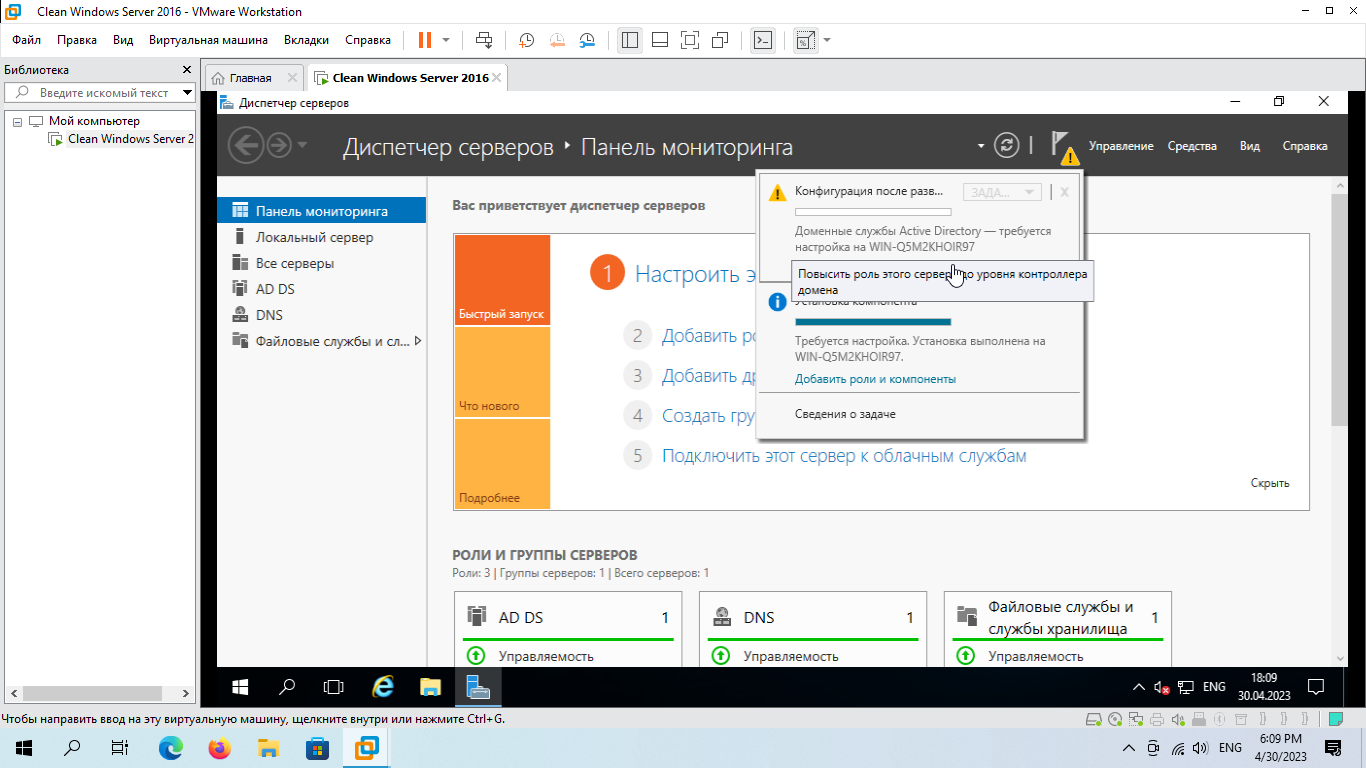
\includegraphics[width=0.85\textwidth]{Screenshot_51}
    \caption{И повышаем роль до уровня контроллера домена}
    \label{img:51}
  \end{figure}

  Контроллеру домена требуется домен, создадим его:

  \begin{figure}[H]
    \centering
    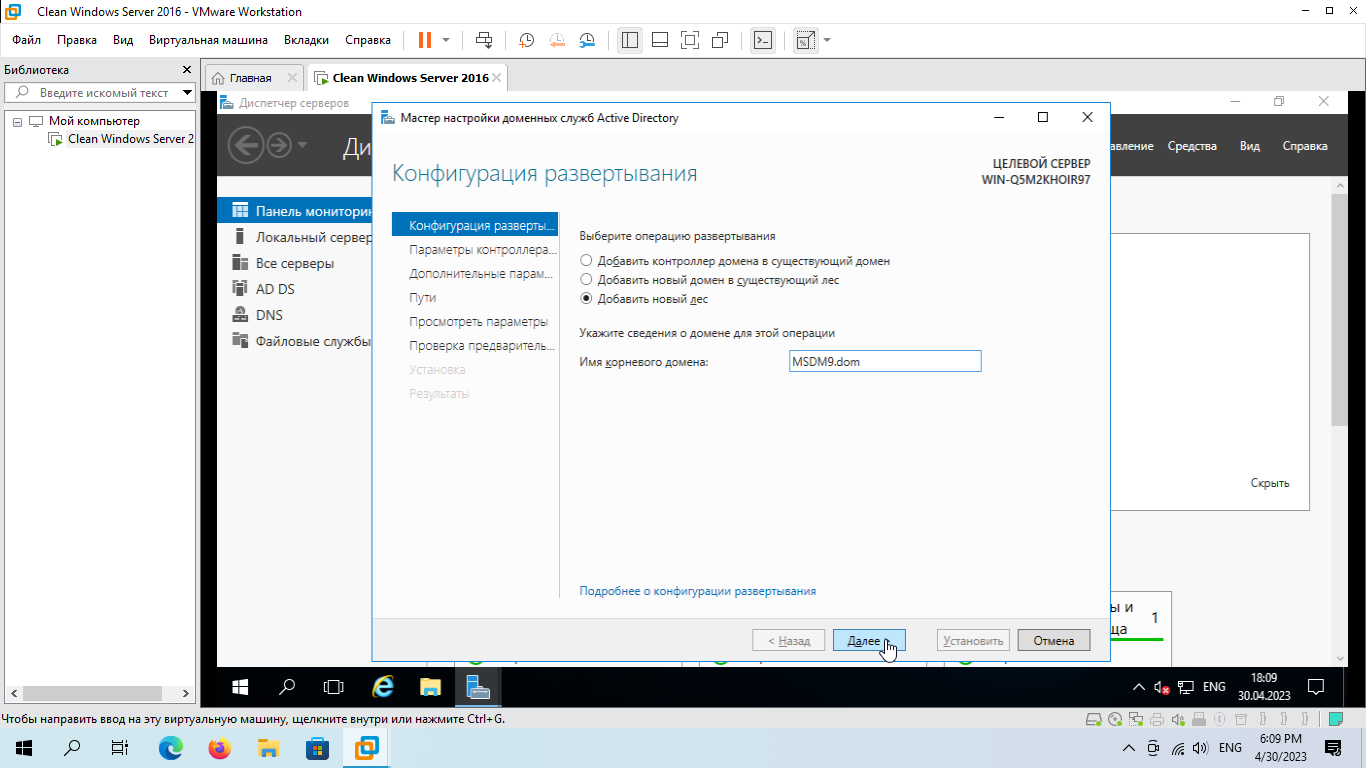
\includegraphics[width=0.85\textwidth]{Screenshot_52}
    \caption{Добавляем новый лес с именем \textit{MSDM9.dom} (в соответсвии с вариантом)}
    \label{img:52}
  \end{figure}

  \begin{figure}[H]
    \centering
    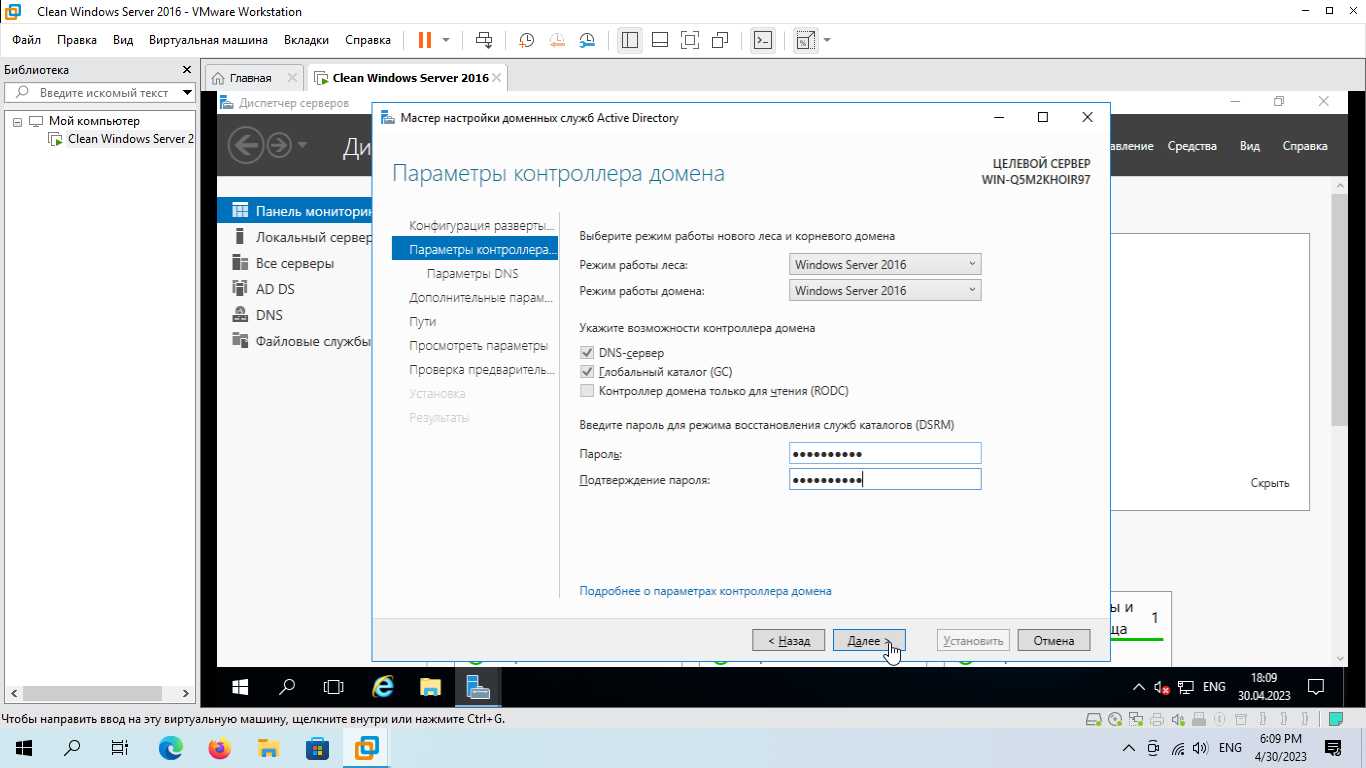
\includegraphics[width=0.85\textwidth]{Screenshot_53}
    \caption{Указываем пароль для режима восстановления}
    \label{img:53}
  \end{figure}

  \begin{figure}[H]
    \centering
    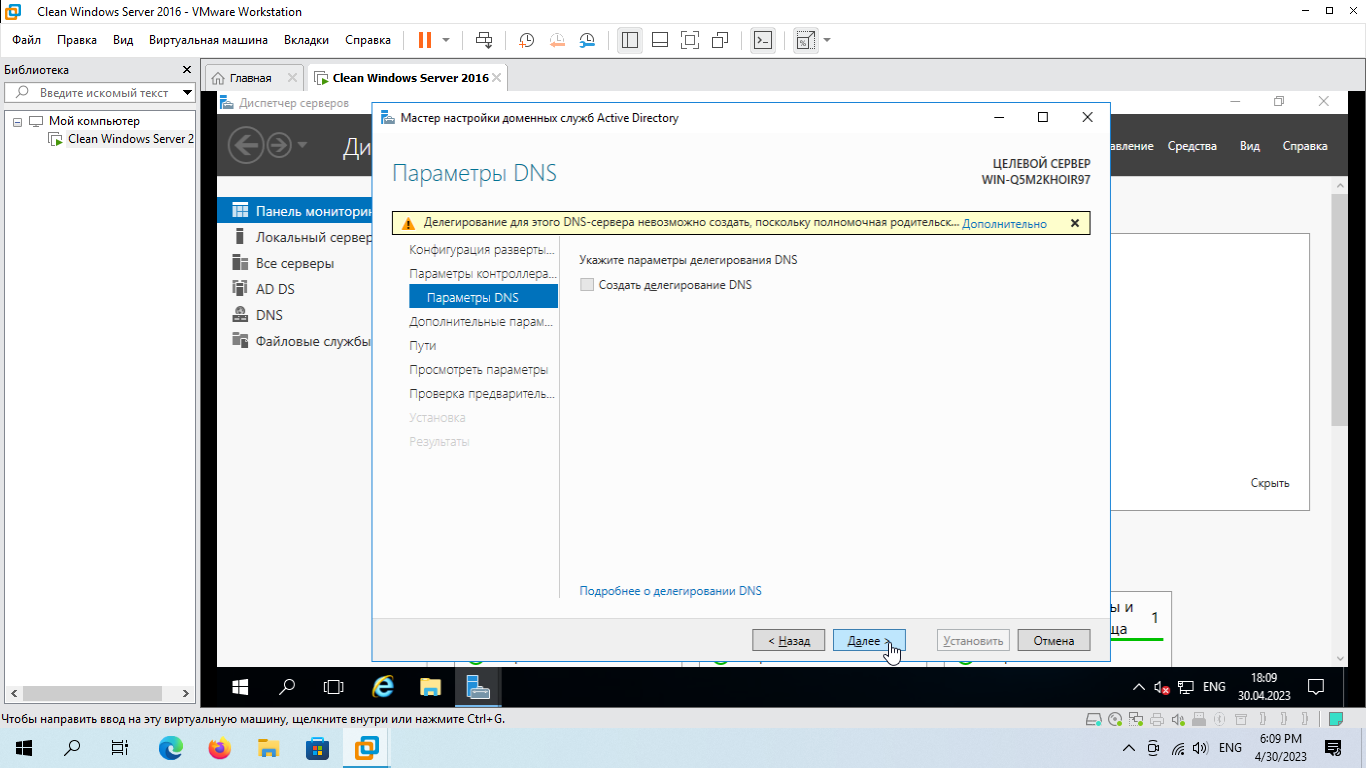
\includegraphics[width=0.85\textwidth]{Screenshot_54}
    \caption{Настройки \textit{DNS} оставляем без изменений}
    \label{img:54}
  \end{figure}

  \begin{figure}[H]
    \centering
    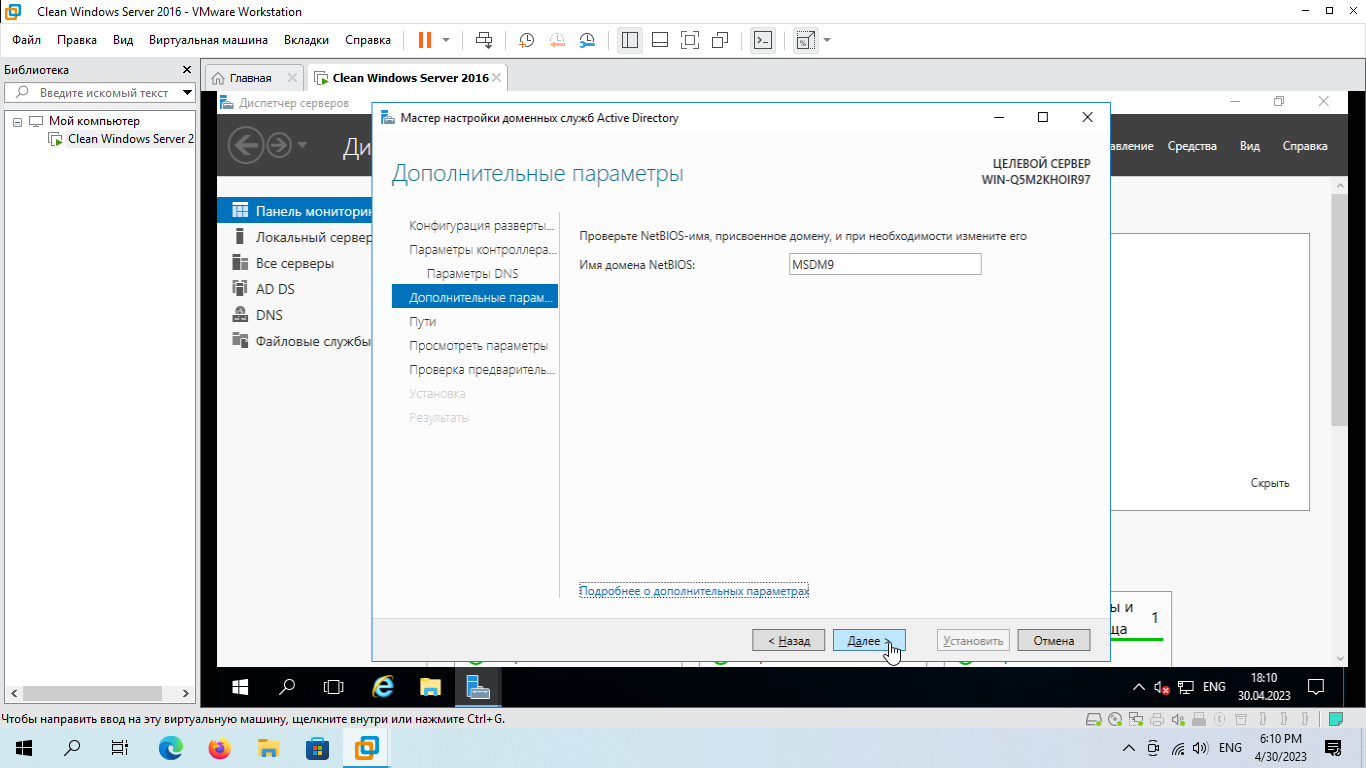
\includegraphics[width=0.85\textwidth]{Screenshot_55}
    \caption{Имя домена само правильно установилось}
    \label{img:55}
  \end{figure}

  \begin{figure}[H]
    \centering
    \includegraphics[width=0.85\textwidth]{Screenshot_56}
    \caption{Пути не изменяем}
    \label{img:56}
  \end{figure}

  \begin{figure}[H]
    \centering
    \includegraphics[width=0.85\textwidth]{Screenshot_57}
    \caption{Проверяем созданную конфигурацию}
    \label{img:57}
  \end{figure}

  \begin{figure}[H]
    \centering
    \includegraphics[width=0.85\textwidth]{Screenshot_58}
    \caption{Приступаем к установке новых изменений}
    \label{img:58}
  \end{figure}

  \begin{figure}[H]
    \centering
    \includegraphics[width=0.85\textwidth]{Screenshot_59}
    \caption{Ждем}
    \label{img:59}
  \end{figure}

  \begin{figure}[H]
    \centering
    \includegraphics[width=0.85\textwidth]{Screenshot_60}
    \caption{Установка завершена - необходима перезагрузка}
    \label{img:60}
  \end{figure}

  \begin{figure}[H]
    \centering
    \includegraphics[width=0.85\textwidth]{Screenshot_61}
    \caption{Выполняется перезагрузка}
    \label{img:61}
  \end{figure}

  \begin{figure}[H]
    \centering
    \includegraphics[width=0.85\textwidth]{Screenshot_62}
    \caption{Заходим в учетную запись пользователя}
    \label{img:62}
  \end{figure}

  \begin{figure}[H]
    \centering
    \includegraphics[width=0.85\textwidth]{Screenshot_63}
    \caption{Необходимо поменять пароль}
    \label{img:63}
  \end{figure}

  Далее необходимо добавить новых пользователей:

  \begin{figure}[H]
    \centering
    \includegraphics[width=0.85\textwidth]{Screenshot_64}
    \caption{Открываем настройки \textit{AD DS} (пункт "Управляемость")}
    \label{img:64}
  \end{figure}

  \begin{figure}[H]
    \centering
    \includegraphics[width=0.85\textwidth]{Screenshot_65}
    \caption{Переходим к самим настройкам}
    \label{img:65}
  \end{figure}

  \begin{figure}[H]
    \centering
    \includegraphics[width=0.85\textwidth]{Screenshot_68}
    \caption{Запускаем "Центр администрирования Active Directory" (через клик ПКМ по запущенному серверу)}
    \label{img:68}
  \end{figure}

  \begin{figure}[H]
    \centering
    \includegraphics[width=0.85\textwidth]{Screenshot_69}
    \caption{Переходим к настройке пользователей}
    \label{img:69}
  \end{figure}

  \begin{figure}[H]
    \centering
    \includegraphics[width=0.85\textwidth]{Screenshot_71}
    \caption{Начинаем создание нового пользователя}
    \label{img:71}
  \end{figure}

  \begin{figure}[H]
    \centering
    \includegraphics[width=0.85\textwidth]{Screenshot_72}
    \caption{Указываем необходимые параметры}
    \label{img:72}
  \end{figure}

  Для пользователя необходимо задать его имя (в соответсвии с вариантом winuser-9-1) и пароль.
  Нужно также создать второго пользователя:

  \begin{figure}[H]
    \centering
    \includegraphics[width=0.85\textwidth]{Screenshot_73}
    \caption{Начинаем создание}
    \label{img:73}
  \end{figure}

  \begin{figure}[H]
    \centering
    \includegraphics[width=0.85\textwidth]{Screenshot_75}
    \caption{Указываем имя пользователя и пароль}
    \label{img:75}
  \end{figure}

  \begin{figure}[H]
    \centering
    \includegraphics[width=0.85\textwidth]{Screenshot_76}
    \caption{Пользователи появились в общем списке}
    \label{img:76}
  \end{figure}

  Теперь домен настроен и готов к работе.

  \subsection{Настройка клиента}

  \subsubsection{Создание ВМ}

  В качестве клиента будет выступать виртуальныя машина с ОС \textit{Widnows 10}.
  Снова возспользуемся заранее подготовленным образом:

  \begin{figure}[H]
    \centering
    \includegraphics[width=0.85\textwidth]{Screenshot_77}
    \caption{Запускаем импорт ВМ}
    \label{img:77}
  \end{figure}

  \begin{figure}[H]
    \centering
    \includegraphics[width=0.85\textwidth]{Screenshot_78}
    \caption{Указываем путь до образа системы}
    \label{img:78}
  \end{figure}

  \begin{figure}[H]
    \centering
    \includegraphics[width=0.85\textwidth]{Screenshot_79}
    \caption{Виртуальная машина создана}
    \label{img:79}
  \end{figure}

  \begin{figure}[H]
    \centering
    \includegraphics[width=0.85\textwidth]{Screenshot_80}
    \caption{Подключим ее к необходимой \textit{NAT} сети}
    \label{img:80}
  \end{figure}

  \begin{figure}[H]
    \centering
    \includegraphics[width=0.85\textwidth]{Screenshot_81}
    \caption{Запускаем ВМ и входим в учетную запись пользователя}
    \label{img:81}
  \end{figure}

  \subsubsection{Настройка сети}

  Необходимо выдать данной машине свой \textit{IP} адрес, указать шлюз  и \textit{DNS}:

  \begin{figure}[H]
    \centering
    \includegraphics[width=0.85\textwidth]{Screenshot_82}
    \caption{Открываем Панель Управления}
    \label{img:82}
  \end{figure}

  \begin{figure}[H]
    \centering
    \includegraphics[width=0.85\textwidth]{Screenshot_83}
    \caption{Переходим во вкладку "Сеть и Интернет"}
    \label{img:83}
  \end{figure}

  \begin{figure}[H]
    \centering
    \includegraphics[width=0.85\textwidth]{Screenshot_84}
    \caption{Открываем центр управления сетями и общим доступом}
    \label{img:84}
  \end{figure}

  \begin{figure}[H]
    \centering
    \includegraphics[width=0.85\textwidth]{Screenshot_86}
    \caption{Выбираем необходимый сетевой адаптер}
    \label{img:86}
  \end{figure}

  \begin{figure}[H]
    \centering
    \includegraphics[width=0.85\textwidth]{Screenshot_87}
    \caption{Переходим к его свойствам}
    \label{img:87}
  \end{figure}

  \begin{figure}[H]
    \centering
    \includegraphics[width=0.85\textwidth]{Screenshot_88}
    \caption{Открывам параметры \textit{IPv4} адреса}
    \label{img:88}
  \end{figure}

  \begin{figure}[H]
    \centering
    \includegraphics[width=0.85\textwidth]{Screenshot_89}
    \caption{Производим настройку}
    \label{img:89}
  \end{figure}

  В качестве \textit{IP} адреса был выбран первый доступный - 192.168.142.3, маска
  подсети не изменилась, шлюз также остался прежним.
  Однако в качестве \textit{DNS} сервера будет использоваться машина с \textit{Windows Server},
  что позводит получать информацию о созданном домене.

  \begin{figure}[H]
    \centering
    \includegraphics[width=0.85\textwidth]{Screenshot_90}
    \caption{Проверяем конфигурацию при помощи \textit{ipconfig}}
    \label{img:90}
  \end{figure}

  \subsubsection{Изменяем имя компьютера}

  Это необходимо для того, чтобы его можно было легче идентифицировать в настройках \textit{Active Directory} в будущем.

  \begin{figure}[H]
    \centering
    \includegraphics[width=0.85\textwidth]{Screenshot_92}
    \caption{Переходим к параметрам системы}
    \label{img:92}
  \end{figure}

  \begin{figure}[H]
    \centering
    \includegraphics[width=0.85\textwidth]{Screenshot_93}
    \caption{Пункт "О программе"}
    \label{img:93}
  \end{figure}

  \begin{figure}[H]
    \centering
    \includegraphics[width=0.85\textwidth]{Screenshot_94}
    \caption{Нажимаем кнопку "Переименовать этот ПК"}
    \label{img:94}
  \end{figure}

  \begin{figure}[H]
    \centering
    \includegraphics[width=0.85\textwidth]{Screenshot_95}
    \caption{Устанавливаем имя в соответсвии с вариантом - windows10-9}
    \label{img:95}
  \end{figure}

  \begin{figure}[H]
    \centering
    \includegraphics[width=0.85\textwidth]{Screenshot_96}
    \caption{Перезагружаем систему, чтобы изменения вступили в силу}
    \label{img:96}
  \end{figure}

  \begin{figure}[H]
    \centering
    \includegraphics[width=0.85\textwidth]{Screenshot_97}
    \caption{Перезагрузка}
    \label{img:97}
  \end{figure}

  \begin{figure}[H]
    \centering
    \includegraphics[width=0.85\textwidth]{Screenshot_98}
    \caption{Снова входим в учетную запись пользователя}
    \label{img:98}
  \end{figure}

  \subsubsection{Подключение к домену}

  Теперь подключим клиентскую машину к домену:

  \begin{figure}[H]
    \centering
    \includegraphics[width=0.85\textwidth]{Screenshot_99}
    \caption{Открываем параметры системы}
    \label{img:99}
  \end{figure}

  \begin{figure}[H]
    \centering
    \includegraphics[width=0.85\textwidth]{Screenshot_100}
    \caption{Пункт "О программе"}
    \label{img:100}
  \end{figure}

  \begin{figure}[H]
    \centering
    \includegraphics[width=0.85\textwidth]{Screenshot_101}
    \caption{Дополнительные параметры системы}
    \label{img:101}
  \end{figure}

  \begin{figure}[H]
    \centering
    \includegraphics[width=0.85\textwidth]{Screenshot_102}
    \caption{Переходим к изменения параметров домена}
    \label{img:102}
  \end{figure}

  \begin{figure}[H]
    \centering
    \includegraphics[width=0.85\textwidth]{Screenshot_104}
    \caption{Вводим имя домена, к которому хотим подсоединиться - MSDM9}
    \label{img:104}
  \end{figure}

  \begin{figure}[H]
    \centering
    \includegraphics[width=0.85\textwidth]{Screenshot_106}
    \caption{Указываем данные учетной записи администратора домена}
    \label{img:106}
  \end{figure}

  \begin{figure}[H]
    \centering
    \includegraphics[width=0.85\textwidth]{Screenshot_107}
    \caption{Подключение к домену произошло успешно}
    \label{img:107}
  \end{figure}

  \begin{figure}[H]
    \centering
    \includegraphics[width=0.85\textwidth]{Screenshot_108}
    \caption{Перезагружаем компьютер}
    \label{img:108}
  \end{figure}

  \begin{figure}[H]
    \centering
    \includegraphics[width=0.85\textwidth]{Screenshot_109}
    \caption{Перезагрузить сейчас}
    \label{img:109}
  \end{figure}

  \subsection{Проверка работоспособности}

  Удостоверимся, что теперь на клиентской машине можно использовать учетные записи,
  созданные и настроенные на сервере:

  \begin{figure}[H]
    \centering
    \includegraphics[width=0.85\textwidth]{Screenshot_110}
    \caption{Укажем логин и пароль для ранее созданного пользователя winuser-9-1}
    \label{img:110}
  \end{figure}

  Видно, что вход осуществляется в необходимый нам домен MSDM9.

  \begin{figure}[H]
    \centering
    \includegraphics[width=0.85\textwidth]{Screenshot_111}
    \caption{Данные введены}
    \label{img:111}
  \end{figure}

  \begin{figure}[H]
    \centering
    \includegraphics[width=0.85\textwidth]{Screenshot_112}
    \caption{Необходимо сменить пароль}
    \label{img:112}
  \end{figure}

  \begin{figure}[H]
    \centering
    \includegraphics[width=0.85\textwidth]{Screenshot_113}
    \caption{Изменяем его}
    \label{img:113}
  \end{figure}

  \begin{figure}[H]
    \centering
    \includegraphics[width=0.85\textwidth]{Screenshot_114}
    \caption{Производится вход в учетную запись}
    \label{img:114}
  \end{figure}

  \begin{figure}[H]
    \centering
    \includegraphics[width=0.85\textwidth]{Screenshot_115}
    \caption{Со мной разговаривает компьютер... А я с ним)}
    \label{img:115}
  \end{figure}

  \begin{figure}[H]
    \centering
    \includegraphics[width=0.85\textwidth]{Screenshot_116}
    \caption{Необходимо удостовериться, что пользователь действительно верный}
    \label{img:116}
  \end{figure}

  \begin{figure}[H]
    \centering
    \includegraphics[width=0.85\textwidth]{Screenshot_117}
    \caption{Посмотрим его параметры}
    \label{img:117}
  \end{figure}

  \begin{figure}[H]
    \centering
    \includegraphics[width=0.85\textwidth]{Screenshot_118}
    \caption{Все верно}
    \label{img:118}
  \end{figure}

  На клиентской машине осуществен вход в доменную учетную запись пользователя.
  Теперь проверим что сервер также знает о клиентской машине:

  \begin{figure}[H]
    \centering
    \includegraphics[width=0.85\textwidth]{Screenshot_119}
    \caption{В настройках AD DS перейдем к списку компьютеров}
    \label{img:119}
  \end{figure}

  \begin{figure}[H]
    \centering
    \includegraphics[width=0.85\textwidth]{Screenshot_120}
    \caption{Клиентский компьютер есть в списке}
    \label{img:120}
  \end{figure}

  \section{Вывод}

  В ходе данной работы я улучшил свои навыки работы с сетью, научился поднимать и настраивать Windows
  Server, а также создавать домен, добавлять в него пользователей и подключать к нему другие машины.

\end{document}
